\documentclass[11pt]{article}
\usepackage[sc]{mathpazo} %Like Palatino with extensive math support
\usepackage{amsmath, amsthm}
\usepackage{fullpage}
\usepackage[authoryear,sectionbib,sort]{natbib}
\linespread{1.7}
\usepackage[utf8]{inputenc}
\usepackage{lineno}
\usepackage{titlesec}
\usepackage{caption, subcaption, multirow, morefloats, rotating}
\usepackage{wrapfig}

\titleformat{\section}[block]{\Large\bfseries\filcenter}{\thesection}{1em}{}
\titleformat{\subsection}[block]{\Large\itshape\filcenter}{\thesubsection}{1em}{}
\titleformat{\subsubsection}[block]{\large\itshape}{\thesubsubsection}{1em}{}
\titleformat{\paragraph}[runin]{\itshape}{\theparagraph}{1em}{}[. ]\renewcommand{\refname}{Literature Cited}

%%%%%%%%%%%%%%%%%%%%%
% Line numbering
%%%%%%%%%%%%%%%%%%%%%
%\usepackage{lineno}
% Please use line numbering with your initial submission and
% subsequent revisions. After acceptance, please turn line numbering
% off by adding percent signs to the lines %\usepackage{lineno} and
% to %\linenumbers{} and %\modulolinenumbers[3] below.

\title{How macroecology affects macroevolution: the interplay between extinction intensity and trait-dependent extinction in brachiopods.}

% This version of the LaTeX template was last updated on
% January 11, 2018.

%%%%%%%%%%%%%%%%%%%%%
% Authorship
%%%%%%%%%%%%%%%%%%%%%
% Please remove authorship information while your paper is under review,
% unless you wish to waive your anonymity under double-blind review. You
% will need to add this information back in to your final files after
% acceptance.

\author{Peter D. Smits$^{1,\ast}$}

\date{}

\begin{document}

\maketitle

\noindent{} 1. University of California -- Berkeley, Berkeley, California 94720;

\noindent{} $\ast$ Corresponding author; e-mail: psmits@berkeley.edu

\bigskip

\textit{Manuscript elements}: 

\bigskip

\textit{Keywords}: species selection, geographic range, environmental preference, paleobiology, Bayesian

\bigskip

\textit{Manuscript type}: Article. %Or e-article, note, e-note, natural history miscellany, e-natural history miscellany, comment, reply, invited symposium, or countdown to 150.

\bigskip

\noindent{\footnotesize Prepared using the suggested \LaTeX{} template for \textit{Am.\ Nat.}}

\linenumbers{}
\modulolinenumbers[3]

\newpage{}

\section*{Abstract}

Trait-based selection is the force behind differences in fitness; the most extreme example of selection being extinction. Modern experiments and observations have shown that average fitness and selection can vary in time and space as environments and interactions change. This begs the question ``as average fitness increases, does the strength of selection increase or decrease?'' The fossil record illustrates that extinction rates have varied through time, with periods of rapid species turnover as well as slow species turnover. With Paleozoic brachiopods as a study system, I developed a model to estimate the average duration of a species (i.e. fitness), how duration varies based on species' biological traits (i.e. selection), and how these evolutionary forces covary. I analyzed how the effects of genus geographic range, preference for epicontinental seas versus open ocean environments, and body size on duration while allowing these effects to vary over time. Environmental preference is presented as a continuum between epicontinental and open-ocean specialists, with degrees of environmental generality in between, so a possibly nonlinear (i.e. quadratic) relationship between environmental preference and duration was modeled. I find evidence that as extinction intensity increases that the magnitude of the effect of geographic range on extinction risk increases, which then increases the difference in extinction risk between small and large ranged taxa during periods of high extinction risk. Similarly, I find strong evidence for a non-linear relationship between environmental preference for epicontinental versus open-ocean environments and expected taxon duration, where taxa with intermediate or no environmental preference are expected to have greater durations than taxa which appear exclusively in either environmental end-member. Finally, I find that taxa which appear more frequently in epicontinental environments will have a greater expected duration than those taxa which prefer open-ocean environments. My analysis supports the conclusions that that as extinction intensity increases and average fitness decreases, as in a mass extinction, the trait-associated differences in fitness (selection) would increase and be greater than aeverage. In contrast, during periods of low extinction intensity when fitness is greater than average, my model predicts that geographic range and environmental preference associated differences in fitness (selection) would decrease and be less than average.

\newpage{}

\section*{Introduction}

% The journal does not have numbered sections in the main portion of
% articles. Please refrain from using section references (à la
% section~\ref{section:CountingOwlEggs}), and refer to sections by name
% (e.g. section ``Counting Owl Eggs'').
Trait-based selection is the force behind differences in fitness; the most extreme example of selection being extinction. Modern experiments and paleontological analyses have demonstrated that selection strength and fitness can vary over time and space. That these evolutionary currencies vary over time begs the question ``do they covary?'' Specifically, how does the strength of selection change as average fitness also changes? The fossil record demonstrates that extinction risk has varied continuously over time, from periods of low average extinction rate to very high extinction rates (e.g. mass extinctions) \citep{Foote2001,Foote2000,Foote2000a}. Paleontological analyses have also demonstrated trait-based differences in extinction risk among taxa \citep{Jablonski2008a}. Conceptually, extinction is the ultimate manifestation of selection as we would expect that a taxon with a beneficial trait to persist for longer than a similar taxon without that trait due to selection \citep{Jablonski2008a,Rabosky2010b,Raup1994,Stanley1975}. Thus, the expected duration of a species can be conceived of as a measure of a species' fitness \citep{Cooper1984}; this then means that trait-associated differences in species fitness are (species) selection \citep{Rabosky2010b}.

In order to test for an association between extinction intensity and extinction selectivity, extinction rate and trait-based differences in extinction rate need to be estimated. Previous work has approached this problem by estimating the extinction intensity and selectivity at different time points or for different origination cohorts independently and then comparing those estimates \citep{Payne2016}. I find this approach problematic for a few reasons.  Modeling each each time point or cohort independently does not use all of the information present in the data and their estimates are only based the data from that time point. A hierarchical/mixed-effect modelling approach leverages all data across time points or cohorts by partially pooling information across each of the time-points or cohorts. The resulting parameter estimates have better behaved posteriors (e.g. smaller credible intervals) and limit spurious parameter estimates by weighing estimates by the amount of data associated with each time point or cohort \citep{Gelman2013d}. Importantly, the partial pooling in hierarchical/mixed-effect also mitigates the effect of complete separation which prevent parameter estimates for some time points or cohorts \citep{Payne2016,Gelman2013d}. Finally, treating each time point or cohort as independent any and all post-hoc analyses are at risk of false positive results due to multiple comparisons \citep{Gelman2007,Gelman2013d}; hierarchical/mixed-effect models ameliorate this problem as possible comparisons are simultaneously modeled.

\citet{Jablonski1986} observed that for bivalves at the end Cretaceous mass extinction event, previous trait-associated differences in survival no longer mattered except for the case of geographic range. Based on this evidence, \citet{Jablonski1986} proposed the idea of "macroevolutionary regimes" and that mass extinction and background extinction are fundamentally different processes. However, based on estimates of extinction rates over time, there is no evidence of there being two or more "types" of extinction \citep{Wang2003}. Instead, extinction rates for marine invertebrates are unimodal with continuous variation. This conflict arises because differences between these papers is that \citet{Jablonski1986} is conidering qualitative differences while \citet{Wang2003} is considering quantitative differences. This disconnect between the theory of macroevolutionary modes and the observation of continuous variation in extinction rates implies the possibility of a relationship between the strength of selection (extinction intensity) and the association between of traits and differences in fitness (extinction selectivity) \citep{Payne2016}. As extinction intensity increases, what happens to extinction selectivity? How do trait-associated differences in fitness change as average extinction rate changes over time?

Here I develop a statistical model describing the relationship between brachiopod taxon durations and multiple functional taxon traits in order to understand the relationship between extinction intensity and selectivity over time. Trait-dependent differences in extinction risk should be associated with differences in taxon duration \citep{Cooper1984,Rabosky2010b}. Brachiopods are an ideal group for this study as they have an exceptionally complete fossil record \citep{Foote1996e,Foote2000a}. I focus on the brachiopod record from the post-Cambrian Paleozoic, from the start of the Ordovician (approximately 485 My) through the end Permian (approximately 252 My) as this represents the time of greatest global brachiopod diversity \citep{Alroy2010} which results in a large sample size.

The analysis of taxon durations, or time from a taxon's origination till its extinction, falls under the purview of survival analysis, a field of applied statistics commonly used in health care and engineering \citep{Klein2003} but has a long history in paleontology \citep{Simpson1944,Simpson1953,VanValen1973,VanValen1979,Smits2015,Crampton2016}. I adopt a hierarchical Bayesian modeling approach \citep{Gelman2007,Gelman2013d} in order to unify the previously distinct dynamic and cohort paleontological survival approaches \citep{VanValen1973,VanValen1979,Raup1978,Raup1975,Foote1988,Baumiller1993,Simpson2006,Crampton2016,Ezard2012b}. 

While estimation of trait-dependent speciation and extinction rates from phylogenies of extant taxa has grown dramatically \citep{Maddison2007,Fitzjohn2010,Goldberg2011a,Goldberg2005,Rabosky2013,Stadler2013b,Stadler2011a,Stadler2013a}, there are two major ways to estimate trait-dependent extinction: analysis of phylogenies, and analysis of the fossil record. These two directions, phylogenetic comparative and paleobiological, are complementary and intertwined in the field of macroevolution \citep{Rabosky2010b,Jablonski2008a,Hunt2014a}. In the case of extinction, analysis of the fossil record has the distinct advantage over phylogenies of only extant taxa because extinction is observable; this means that extinction rate is possible to estimate \citep{Rabosky2010a,Quental2009,Liow2010a}. The approach used here is thus complementary to the analysis of trait-dependent extinction based on a phylogeny.

\subsection*{Factors affecting brachiopod survival}

Conceptually, taxon survival can be considered an aspect of ``taxon fitness'' \citep{Cooper1984,Palmer2012}. Traits associated with taxon survival are thus examples of species (or higher-level) selection, as differences in survival are analogous to differences in fitness. The traits analyzed here are all examples of emergent and aggregate traits \citep{Jablonski2008a,Rabosky2010b}; specifically I analyze genus-level traits. Emergent traits are those which are not measurable at a lower level (e.g. species versus individual organism) such as geographic range, or even fossil sampling rate. Aggregate traits, like body size or environmental preference, are the average of a shared trait across all members of a lower level.

Geographic range is widely considered the most important biological trait for estimating differences in extinction risk at nearly all times, with large geographic range associated with low extinction risk \citep{Jablonski1986,Jablonski1987,Jablonski2003,Payne2007,Jablonski2008a,Harnik2013,Finnegan2012a}. This stands to reason even if extinction is completely at random; a taxon with a broad range is less likely to go extinct at random than a taxon with a restricted range.

Epicontinental seas are a shallow-marine environment where the ocean has spread over the continental interior or craton with a depth typically less than 100m. In contrast, open-ocean coastline environments have much greater variance in depth, do not cover the continental craton, and can persist during periods of low sea level \citep{Miller2009a}. Because of this, a simple hypothesis that taxa which favor epicontinental seas would be at great risk during periods of low sea levels, such as during glacial periods, when epicontinental seas are drained. During the Paleozoic (approximately 541--252 My), epicontinental seas were widely spread globally but declined over the Mesozoic (approximately 252--66 My) and have nearly disappeared during the Cenozoic (approximately 66--0 My) as open-ocean coastlines became the dominant shallow-marine setting \citep{Sheehan2001b,Peters2008,Miller2009a,Johnson1974}. Taxa in epicontinental environments could also have a greater extinction susceptibility than taxa in open-ocean environments due to anoxic events due to enhanced water stratification or poor water circulation \citep{Peters2007}.

\citet{Miller2009a} demonstrated that during several mass extinctions taxa associated with open-ocean environments tend to have a greater extinction risk than those taxa associated with epicontinental seas. During periods of background extinction, however, they found no consistent difference between taxa favoring either environment. \citet{Miller2009a} hypothesize that open-ocean taxa may have a greater extinction rate because these environments would be more strongly affected by poisoning of the environment from impact fallout or volcanic events because water circulates at a higher rate and in greater volume in open-ocean environments compared to the relatively more sluggish ciruclation in epicontinental environments. These two environment types represent the primary identifiable environmental dichotomy observed in ancient marine systems \citep{Miller2009a,Sheehan2001b}. Given these findings, I would hypothesize that as extinction risk increases, the extinction risk associated with open-ocean environments should generally increase. 

Because environmental preference is defined here as the continuum between occurring exclusively in open-ocean environments versus epicontinental environments, intermediate values are considered ``generalists'' in the sense that they favor neither end member. A long-standing hypothesis is that generalists or unspecialized taxa will have greater survival than specialists \citep{Simpson1944,Liow2004a,Liow2007b,Nurnberg2013a,Nurnberg2015,Baumiller1993,Smits2015}. Because of this, the effect of environmental preference was modeled as a quadratic function where a concave down relationship between preference and expected duration indicates that generalists are favored over specialists end-members. Importantly, this approach does not ``force'' a non-linear relationship, and only allows one if the second-order term is non-zero.

Body size, measured as shell length, is also considered as a trait that may potentially influence extinction risk \citep{Payne2014,Harnik2011}. Body size is a proxy for metabolic activity and other correlated life history traits \citep{Payne2014}. \citet{Harnik2014} analyzed the effect of body size selectivity in Devonian brachiopods in a phylogenetic and non-phylogenetic context; finding that body size was not found to be associated with differences in taxonomic duration. It has also been found that, at least in the case of some bivalve subclades, body size can be as important a factor as geographic range size in determining extinction risk \citep{Harnik2011}. Given these results, I expect that if body size has any effect on brachiopod taxonomic survival it is very small.

It is well known that, given the incompleteness of the fossil record, the observed duration of a taxon is an underestimate of that taxon's true duration \citep{Solow1997,Wagner2013a,Wang2004,Liow2010b,Alroy2014a,Foote1996e}. Because of this, the concern is that a taxon's observed duration may reflect its relative chance of being sampled and not any of the effects of the covariates of interest. In this case, for sampling to be a confounding factor there must be consistent relationship between the quality of sampling of a taxon and its apparent duration (e.g. greater sampling, longer duration). If there is no relationship between sampling and duration then interpretation can be made clearly; while observed durations are obviously truncated true durations, a lack of a relationship would indicate that the amount and form of this truncation is not a major determinant of the taxon's apparent duration. By including sampling as a covariate in the model, this effect can be quantified and can be taken into account when interpreting the estimates of the effects of the other covariates.


%\begin{table}[h]
%  \centering
%  \caption{Primary analytical questions tested using this model}
%  \begin{tabular}{l l l}
%    Question & Possible results and explanation & Sources
%    \hline
%    Relationship between geographic range and duration & positive relationship (predicted), no relationship, negative relationship (unlikely) & \\
%    Relationship between environmental preference and duration & non-linear concave down (predicted), linear with slope != 0, linear with slope == 0 (unlikely) & \\
%    Correlation between average cohort duration and effect of geographic range on duration & positive correlation (duration inc, effect inc), negative correlation (duration inc, effect desc) & \\
%    Correlation between average cohort duration and environmental preference (linear term) & & \\
%    Correlation between average cohort duration and environmental preference (squared term) & & \\
%    Correlation between effect of geographic range and effect of environmental preference (linear term) & & \\
%    Correlation between effect of geographic range and effect of environmental preference (squared term) & & \\
%  \end{tabular}
%  \label{tab:hypo}
%\end{table}




\section*{Methods}

% foote gave me a hand with the taxonomic occurrences
%   biggest limiting factor is the Payne 2014 body size dataset
The brachiopod dataset analyzed here was sourced from the Paleobiology Database (http://www.paleodb.org) and then filtered to a limited selection of higher taxonomic groups (Rhychonelliformea: Rhynchonellata, Chileata, Obolellida, Kutorginida, Strophomenida, Spiriferida). Additionally, samples were limited to those taxa present during the post-Cambrian Paleozoic. Temporal, stratigraphic, and other relevant occurrence information used in this analysis was also downloaded. Analyzed occurrences were restricted to those with paleolatitude and paleolongitude coordinates, have been assigned to either epicontinental or open-ocean environment, and belonging to a genus present in the body size dataset \citep{Payne2014}. Epicontinental versus open-ocean assignments for each fossil occurrence are based on those from previous analyses \citet{Miller2009a,Foote2013,Ritterbush2017}. These filtering criteria are very similar to those from \citet{Foote2013} with an additional constraint of being present in the body size data set from \citet{Payne2014}. In total, there 1130 genera were included in this analysis.

% justification of using genus level versus specific
Fossil occurrences were analyzed at the genus level, a common proactice for paleobiological, macroevolutionary and macroecological studies and this is especially the case for marine invertebrates \citep{Alroy2010,Foote2013,Harnik2013,Kiessling2007a,Miller2009a,Nurnberg2013a,Nurnberg2015,Payne2007,Ritterbush2017,Simpson2009,Vilhena2013,Eronen2011a}. While species diversity dynamics are frequently of much greater interest than those of higher taxa (though see \citealt{Foote2014b,Hoehn2015}), the nature of the fossil record makes accurate, precise, and consistent taxonomic assignments at the species level difficult for all occurrences. As such, the choice to analyze genera as opposed to species was in order to assure a minimum level of confidence and accuracy in the data analyzed here. Additionally, when species and genera can be compared, they often yield similar results \citep{Roy1996,Jernvall2002,Foote2007}. Importantly, it may also be possible genera may represent coherent biological units as there is evidence for congruence between morphologically and genetically defined genera of molluscs and mammals \citep{Jablonski2009}.

Genus duration was calculated as the number of geologic stages from first appearance to last appearance, inclusive. Durations were based on geologic stages as opposed to millions of years because of the inherently discrete nature of the fossil record; dates are not assigned to individual fossils themselves but instead fossils are assigned to a geological interval which represents some temporal range. In this analysis, stages are effectively irreducible temporal intervals in which taxa may occur. Genera with a last occurrence in or after Changhsingian stage (e.g. the final stage of the study interval) were right-censored. Censoring in this context indicates that the genus was observed up to a certain age but its ultimate time of extinction is unknown \citep{Klein2003}.

The covariates of duration included in this analysis are geographic range size (\(r\)), environmental preference (\(v, v^{2}\)), shell length (\(m\)) and sampling (\(s\)).

A genus's geographic range was calculated as the number of occupied grid cells from a gridded map of all contemporaneous occurrences. First, the paleolatitude-paleolongitude coordinates for all occurrences were projected onto an equal-area cylindrical map projection. Each occurrence was then assigned to one of the cells from a 70 \(\times\) 34 regular raster grid placed on the map. Each grid cell represents approximately 250,000 km\(^{2}\). The map projection and regular lattice were made using shape files from http://www.naturalearthdata.com/ and the \texttt{raster} package for R \citep{raster}. For each stage, the total number of occupied grid cells was calculated. Then, for each temporal bin, the relative occurrence probability of the observed taxa was calculated using the \uppercase{jade} method developed by \citet{Chao2015a}. This method accounts for the fact that taxa with an occupancy of 0 cannot be observed which means that occupancy follows a truncated Binomial distribution. This correction is critical when comparing occupancies from different times with different geographic sampling. Finally, for each genus, the mean relative occurrence probability was calculated as the average of that genus' occurrence probabilities for all stages it was sampled to yield relative occupancy, my proxy for geographic range.

The environmental preference for a taxon is defined by their relative occurrences in epicontinental or open-ocean environments, presenting a continuum from exclusive occurrence at the ends and equal occurrences in the middle. Mathematically, environmental preference was defined as probability of observing the ratio of epicontinental occurrences to total occurrences (\(\theta_{i} = e_{i} / E_{i}\)) or greater given the background occurrence probability \(\theta^{\prime}_{i}\) as estimated from all other taxa occurring at the same time (\(e^{\prime}_{i} / E^{\prime}_{i}\)). This measure of environmental preference is expressed.
\begin{equation}
  \begin{aligned}
    p\left(\theta^{\prime}_{i} \middle| e^{\prime}_{i}, E^{\prime}_{i} \right) &\propto \mathrm{Beta}(e^{\prime}_{i}, E^{\prime}_{i} - e^{\prime}_{i}) \mathrm{Beta}(1, 1) \\
    &= \mathrm{Beta}(e^{\prime}_{i} + 1, E^{\prime}_{i} - e^{\prime}_{i} + 1),
  \end{aligned}
  \label{eq:envpref}
\end{equation}
where \(v\) is the percent of the distribution defined in equation~\ref{eq:envpref} less than or equal to \(\theta_{i}\). The Beta distribution is used here because it is a continuous distribution bounded at 0 and 1, which is idea for modeling percentages.

Body size, measured as shell length, was sourced directly from \citet{Payne2014}. These measurements were made from brachiopod taxa figured in the \textit{Treatise on Invertebrate Paleontology} \citep{Brunton2007}.

The sampling probability for individual taxa, called \(s\) was calculated using the standard gap statistic \citep{Foote1996e,Foote2000}. The gap statistic is calculated as the number of stages in which the taxon was sampled except for its first stage and last stage. Because taxa that were right censored only include a first appearance, one was subtracted from the numerator and denominator instead of two. The inclusion of genus-specific sampling probability as a covariate in the model implicitly deals with my using stratigraphic range as a proxy for genus duration. The implications of this choice are discussed further later in the Discussion.

The minimum duration for which a gap statistic can be calculated is three stages, so I chose the impute the gap statistic for all observations with a duration less than 3. Imputation is the ``filling in'' of missing observations based on the observed values \citep{Rubin1996,Gelman2007}.

Prior to analysis, geographic range was logit transformed and the number of samples was natural-log transformed; these transformations make these variables defined for the entire real line. Sampling probability was transformed as \((s (n - 1) + 0.5) / n\) where \(n\) is the sample size as recommended by \citet{Smithson2006}; this serves to slightly shrink the range of the data so that there are no values of 0 or 1. All covariates except for sampling were standardized by subtracting the mean from all values and dividing by twice its standard deviation, which follows \citet{Gelman2007}. This standardization means that the associated regression coefficients are comparable as the expected change per 1-unit change in the rescaled covariates. Finally, \(D\) is defined as the total number of covariates, excluding sampling, plus one for the intercept term.



\subsection*{Details of model}

% hierarchical modeling is simply modeling the hyperparameters of a prior distribution
%   Gelman2013d
% observed outcomes are conditioned on certain parameters which are themselves modeled
Hierarchical modelling is a statistical approach which explicitly takes into account the structure of the observed data in order to model the within and the between group variances \citep{Gelman2013d,Gelman2007}. The units of study (e.g. genera) each belong to a single group (e.g. origination cohort). Each group is considered a draw from a shared probability distribution (e.g. prior) of all cohorts, observed and unobserved. The group-level parameters, or the hyperparameters of this shared prior, are themselves given (hyper)prior distributions and are also estimated like the other parameters of interest (e.g. covariate effects) \citep{Gelman2013d}. The subsequent estimates are partially pooled together, where parameters from groups with large samples or effects remain large while those of groups with small samples or effects are pulled towards the overall group mean. All covariate effects (regression coefficients), as well as the intercept term (baseline extinction risk), were allowed to vary by group (origination cohort). The covariance between covariate effects was also modeled. 

Genus durations were assumed to follow a Weibull distribution which allows for age-dependent extinction \citep{Klein2003}: \(y \sim \mathrm{Weibull}(\alpha, \sigma)\). The Weibull distribution has two parameters: scale \(\sigma\), and shape \(\alpha\). When \(\alpha = 1\), \(\sigma\) is equal to the expected duration of any taxon. \(\alpha\) is a measure of the effect of age on extinction risk where values greater than 1 indicate that extinction risk increases with age, and values less than 1 indicate that extinction risk decreases with age. Note that the Weibull distribution is equivalent to the exponential distribution when \(\alpha = 1\). 

Censoring and truncation reflects a number of factors that limit our ability to fully observe a taxon's duration: limited resolution, which leads to left-censoring or truncation; end of study interval, which leads to right censoring; and incomplete sampling, which can left-censor (short-lived taxa are less likely to be preserved at all) or right-censor (durations are truncated). You are talking only about the first two sources, which is fine. But it might make sense to state this explicitly and to say that you are dealing with sampling-related censoring by using empirically estimated sampling rates as a predictor in your model.
In the case of the right- and left-censored observations mentioned above, the probability of those observations has a different calculation \citep{Klein2003}. For right-censored observations, the likelihood is calculated \(p(y | \theta) = 1 - F(y) = S(y)\) where \(F(y)\) is the cumulative distribution function. Taxa that existed for only a single stage were left-censored, which implies that that taxon went extinct at any point between 0 and 1 stages. In contrast to right-censored data, the likelihood of a left-censored observation is calculated from \(p(y | \theta) = F(y)\). This censoring strategy improves model fit greatly over treating these taxa as being fully observed; additionally, a model with censoring yields better WAIC and LOOIC values than a model without censoring, which means that the model with censoring is expected to have greater out-of-sample predictive accuracy than the model without censoring (not shown).

The scale parameter \(\sigma\) was modeled as a regression following \citet{Kleinbaum2005} with varying intercept and varying slopes and the effect of sampling; this is expressed
\begin{equation}
  \sigma_{i} = \exp\left(\frac{-\mathbf{X}_{i} B_{j[i]} + \delta s_{i}}{\alpha}\right)
  \label{eq:sigma}
\end{equation}
where \(i\) indexes across all observations where \(i = 1, \dots, n\) where \(n\) is the total number of observations, \(j[i]\) is the cohort membership of the \(i\)th observation where \(j = 1, \dots, J\) where \(J\) is the total number of cohorts, \(X\) is a \(N \times D\) matrix of covariates along with a column of ones for the intercept term, \(B\) is a \(J \times D\) matrix of cohort-specific regression coefficients, and \(\delta\) is the regression coefficient for the effect of sampling \(s\). \(\delta\) does not vary by cohort.

Each of the rows of matrix \(B\) are modeled as realizations from a multivariate normal distribution with length \(D\) location vector \(\mu\) and \(J \times J\) covariance matrix \(\Sigma\): \(B_{j} \sim \mathrm{MVN}(\mu, \Sigma)\). The covariance matrix was then decomposed into a length \(J\) vector of scales \(\tau\) and a \(J \times J\) correlation matrix \(\Omega\), defined \(\Sigma = \mathrm{diag}(\tau) \Omega \mathrm{diag}(\tau)\) where ``diag'' indicates a diagonal matrix.

The elements of \(\mu\) were given independent normally distributed priors. The effects of geographic range size  and the breadth of environmental preference were given informative priors reflecting the previous findings while the others were given weakly informative favoring no effect. The correlation matrix \(\Omega\) was given an LKJ distributed prior \citep{Lewandowski2009} that slightly favors an identity matrix as recommended by \citet{StanManual}. These priors are defined
\begin{equation}
  \begin{aligned}
    \mu^{0} &\sim \mathcal{N}(0, 5) \\
    \mu^{r} &\sim \mathcal{N}(-1, 1) \\
    \mu^{v} &\sim \mathcal{N}(0, 1) \\
    \mu^{v^{2}} &\sim \mathcal{N}(1, 1) \\
    \mu^{m} &\sim \mathcal{N}(0, 0.5) \\
    \delta &\sim \mathcal{N}(1) \\
    \tau &\sim \mathrm{C^{+}}(1) \\
    \Omega &\sim \text{LKJ}(2).
  \end{aligned}
  \label{eq:sigma_prior}
\end{equation}

The log of the shape parameter \(\alpha\) was given a weakly informative prior \(\log(\alpha) \sim \mathcal{N}(0, 1)\) centered at \(\alpha = 1\), which corresponds to the Law of Constant Extinction \citep{VanValen1973}.

\subsection*{Imputation of sampling probability}
% Unknown values were estimated from the results of that beta regression.
The vector sampling \(s\) has two parts: the observed part \(s^{o}\), and the unobserved part \(s^{u}\). Of the 1130 total observations, 539 have a duration of 3 or more and have an observed gap statistic. The gap statistic for the remaining 591 observations was imputed. As stated above, the unobserved part is the imputed, or filled in, based on the observed part \(s^{o}\). Because sampling varies between 0 and 1, I chose to model it as a Beta regression with matrix \(W\) being a \(N \times (D - 3)\) matrix of covariates (i.e. geographic range size, environmental preference, body size; no interactions) as predictors of sampling; this assumes that the sampling value for all taxa come from the same distribution. Importantly, I make no assumptions of causal structure. 

Predicting sampling probability using the other covariate that are then included in the model of duration is acceptable and appropriate in the case of imputation where the sample goal is accurate prediction \citep{Rubin1996,Gelman2007}. Not including these covariates can lead to biased estimates of the imputed variable; if the covariates themselves are related, not including them will bias this correlation towards zero which then leads to improper imputation and inference \citep{Rubin1996}.

The Beta regression is defined
\begin{equation}
  s^{o} \sim \mathrm{Beta}(\phi = \text{logit}^{-1}(X^{o} \gamma), \lambda),
  \label{eq:impute}
\end{equation}
where \(\gamma\) is a length \(D\) vector of regression coefficients, and \(X\) defined as above. The Beta distribution used in the regression is reparameterized in terms of a mean parameter
\begin{equation}
  \phi = \frac{\alpha}{\alpha + \beta}
\end{equation}
and total count parameter
\begin{equation}
  \lambda = \alpha + \beta
\end{equation}
where \(\alpha\) and \(\beta\) are the characteristic parameters of the Beta distribution \citep{Gelman2013d}.

The next step is to then estimate \(s^{u} | s^{o}, X^{o}, X^{u}, \gamma\), the posterior distribution of which are folded back into \(s\) and used as a covariate of duration (Eq.~\ref{eq:sigma}). All the elements of \(\gamma\), \(\delta\) (Eq.~\ref{eq:sigma}), and \(\lambda\) (Eq.~\ref{eq:impute}) were given weakly informative priors as recommended by \citet{StanManual}:
\begin{equation}
  \begin{aligned}
    \gamma &\sim \mathcal{N}(0, 1) \\
    \delta &\sim \mathcal{N}(0, 1) \\
    \lambda &\sim \mathrm{Pareto}(0.1, 1.5). \\
  \end{aligned}
\end{equation}

The imputed values are estimated simultaneously at the same time and in the same manner as other parameters are estimated; this ensures that all uncertainty surrounding these unobservable covariate values is propagated through to all estimates.

\subsection*{Posterior inference and posterior predictive checks}

The joint posterior was approximated using a Markov-chain Monte Carlo routine that is a variant of Hamiltonian Monte Carlo called the No-U-Turn Sampler \citep{Hoffman2014} as implemented in the probabilistic programming language Stan \citep{2014stan}. The posterior distribution was approximated from four parallel chains run for 40,000 steps, split half warm-up and half sampling and thinned to every 20th sample for a total of 4000 posterior samples. Starting conditions for sampling were left at defaults for CmdStan interface except for the following changes: adapt delta was set 0.95 to ensure no divergent samples, and initial value was set to 0 which allows for stable initial samples. Posterior convergence was assessed using standard MCMC diagnostics such as the scale reduction factor \(\hat{R}\) (target \(<1.1\)) and effective sample size or ESS (target eff/steps \(<0.0001\)), and HMC specific criteria such as energy (target \(>0.2\)), presence and number of divergent samples and number of samples that saturated the maximum trajectory length for avoiding infinite loops (target value 0), For futher explanation of these diagnostic criteria, see the Stan Manual \citep{StanManual}.

After the model was fit to the data, 100 datasets were simulated from the posterior predictive distribution of the model. These simulations were used to test for adequacy of model fit as described below.

% simulating 
%  have to be equal to or less than what we actually observed
%  probably have poor fit to the censored observations
Survival analysis is complicated by censored observations where the ultimate time of extinction for some taxa could not be fully observed during the study window. Importantly, posterior predictive simulations for these observations must be similarly censored. To accomplish this, posterior predictive simulated durations for right-censored observations were the minimum of its final observed duration and the simulated duration. For left-censored individuals, their simulated duration was pegged at a minimum of one stage with simulated values less than one stage set to one.

Model adequacy was evaluated using a series of posterior predictive checks. Posterior predictive checks are a means for understanding model fit or adequacy. The concept of model adequacy is that if our model is an adequate descriptor of the observed data, then data simulated from the posterior predictive distribution should be similar to the observed given the same covariates, etc. \citep{Gelman2013d}. Posterior predictive checks can take many forms but the basic idea is to compare some property of the empirical data to that property estimated from each of the simulated datasets. Additionally, for structured datasets like the one analyzed here, the fit of the model to different parts of the data can be assessed, which in turn can reveal a great deal if the model has good fit to some aspects of data but not others; it is in these scenarios when knowledge about the biology, geology, and paleoenvironment becomes important in order to explain what unmodeled processes might lead to these discrepancies between our data and the model \citep{Gelman2013d}.

The types of posterior predictive tests used in this analysis fall into two categories: comparison of observed mean and median genus duration to a distribution of mean and median genus duration estimates from the posterior simulations, comparison of a non-parametric estimate of the survival function from the observed data to estimates of that same survival function from the simulations. 

The survival function describes the probability of a taxon persisting given that it has survived up to time \(t\); this is expressed \(P(T \geq t)\) because \(T\) is the true extinction time of the species and \(t\) is some arbitrary time of observation and we are estimating that probability that \(t\) is less than \(T\). It is important to note, however, that the survival function does not reflect density of observations unlike e.g. histograms. Instead, this posterior predictive check reflects the model's ability to predict genus survival.

These posterior predictive tests were done for the entire data and for each of the origination cohorts.

% everything is on zenodo if you want to reproduce this entire analysis
% All code necessary to reproduce this analysis are available through an archived Zenodo repository DOI URL.






\section*{Results}
I first present the results of the multiple posterior predictive checks for the whole dataset as well as each of the origination cohorts. I next present the parameter posterior estimates and their interpretations. Importantly, the adequacy of model fit associated with each cohort-specific interpretation is presented to demonstrate which results for which I have the greatest confidence.

%\subsection*{Model adequacy and posterior predictive checks}
% total group

Comparisons between the observed distribution of durations to the distributions of 100 simulated datasets reveals the relatively good but heterogeneous fit of the model to the data (Fig.~\ref{fig:dens_overlay_zoom}). The two major aspects of possible misfit that are observable are at at durations of 2-3 stages. The model slightly under-estimates the number of observations with duration of 2 or 3 stages. The goal of this model is estimating the expected duration of a genus given its covariate information. While the model estimates are not exact, it is possible that our model fits the bulk of our data well but does poorly towards the tails. 

Comparisons between the survival functions estimated from the empirical data and from 100 simulated datasets further expands the picture of model adequacy (Fig.~\ref{fig:surv}). The survival curves of the 100 simulated datasets are very similar to the survival function estimated from the empirical data. The major points of potential misfit between the model and the data are underestimated percentage of taxa with duration 1 stage, and an over-estimate of probability of species surviving at least 10-13 stages. Importantly, the major divergence between the observed and estimated applies to taxa with a less than 15\% probability of continuing to surviving. Keep in mind, also, that the survival curve as presented does not depict density of observations as in Fig.~\ref{fig:dens_overlay_zoom}.

In addition to distributional comparisons, model adequacy at the total data level was assessed through comparison of the mean and median of the observed data to those from simulated data sets. While the previous posterior predictive checks have focused on the relatively good but heterogeneous fit of the model to the entire distribution of the data, the fitted model's ability to predict the mean and median of the observed data appears adequate (Fig.~\ref{fig:ppc_mean},~\ref{fig:ppc_median}). Because the principle goal of this model is to obtain adequate prediction of how a taxon's expected duration for a given set of ecological covariates, the seemingly adequate fit of our model to mean taxon duration is reassuring (Fig.~\ref{fig:ppc_mean}). Additionally, given the skewness of the observed taxon durations (Fig.~\ref{fig:dens_overlay_zoom}, the ability for the model to closely recapitulates the median observed taxon duration points to the overall good fit of the model to the data.

When considered together, all of the above posterior predictive checks indicate adequate model fit for key questions such as expected taxon duration (Fig.~\ref{fig:ppc_mean}). However, there is obviously heterogeneity in model fit because, while the model can recapitulate some aspects of the observed data (Fig.~\ref{fig:ppc_mean},~\ref{fig:ppc_median}), there are obvious discrepancies between the model and the data (Fig.~\ref{fig:dens_overlay_zoom},~\ref{fig:surv}). By performing the same posterior predictive tests for each of the origination cohorts, it may be possible to get a better picture of the sources of model misfit.

When the posterior predictive tests are visualized for each of the origination cohorts, a complex picture of model fit emerges. Comparison between the empirical survival functions estimated for each cohort to those estimated from the simulated datasets reveals the degree of heterogeneity in model fit (Fig.~\ref{fig:surv_group}, as some origination cohorts appear to be very well fit by the model (e.g. Tremadoc, Darriwilian Wenlock, Ludlow, Lochkovian, etc.) while others are more poorly fit by the model (e.g. Tournaisian, Visean, Bashirian, Moscovian, Stephanian, Asselian, etc.). The poor model fit to some origination cohorts may indicate that these cohorts are undergoing a different extinction process whose aspects are unmodeled in this analysis. However, for those cohorts where the model recapitulates the empirical survival function it is likely that the model may be capturing some of the processes underlying taxon extinction.

For nearly every origination cohort, the model is able to approximately recapitulate the observed mean duration (Fig.~\ref{fig:group_mean}). In comparison, the model has a much more heterogeneous fit to each origination cohort's median taxon duration (Fig.~\ref{fig:group_median}). The skewness of the distribution underlying (Fig.~\ref{fig:dens_overlay_zoom}) means that for some origination cohorts, median duration might be pegged at 1 stage; this means that the posterior predictive distributions for some cohorts can be extremely skewed. The cohorts with notably inadequate poor predictions are the Hirnantian, Priodoli, Emsian, Eifelian, Givetian, Asselian, Artinskian, and Roadian. The remaining cohorts, however, have adequate fit. These results indicate that our model is very good at recapitulate mean taxon duration (Fig.~\ref{fig:ppc_mean},~\ref{fig:group_mean}), and it is capable of estimating overall median duration and median duration of most origination cohorts (Fig.~\ref{fig:ppc_median},~\ref{fig:group_median}).

A larger than average geographic range is expected to have a positive effect on taxon survival (Table~\ref{tab:param}). The cohort-level estimate of the effect of geographic range size indicates that as a taxon's geographic range increases, that taxon's duration is expected to increase (Table~\ref{tab:param}). Given the estimates of \(\mu^{r}\) and \(\tau^{r}\), there is an approximately 3.7\% (\(\pm 4.3\%\) SD) probability that this relationships would be reversed (\(\mathrm{Pr}\mathcal{N}(\mu^{r}, \tau^{r}) > 0)\)). 

Body size measured as valve length is estimated to, on average, have no effect on duration (Table~\ref{tab:param}).

The group-level estimate of the effect of environmental preference is estimated from \(\mu^{v}\) and \(\mu^{v^{2}}\). The estimate of \(\mu^{v}\) indicates that taxa which slightly prefer epicontinental environments to open-ocean environments are expected to have a greater duration than open-ocean favoring taxa (Table~\ref{tab:param}). Additionally, given the estimate of between-cohort variance \(\tau^{v}\), there is approximately 18.1\% (\(\pm 7.5\%\) SD) probability that, for any given cohort, taxa which favor open-ocean environments would have a greater expected duration than taxa which favor epicontinental environments (\(\mathrm{Pr}(\mathcal{N}(\mu^{v}, \tau^{v}) > 0)\)). The estimate of \(\mu^{v^{2}}\) indicates that the overall relationship between environmental preference and \(\log(\sigma)\) is concave down (Fig.~\ref{fig:env_mean}), with only a 2.5\% (\(\pm 2.9\%\) SD) probability that any given cohort is convex up (\(\mathrm{Pr}(\mathcal{N}(\mu^{v^{2}}, \tau^{v^{2}}) < 0\)).

The cohort-specific estimates of all the regression coefficients demonstrate a lot of between cohort variance, with no obvious long-term trends (Fig.~\ref{fig:cohort_series}). While most cohort-specific estimates are very similar to the overall cohort-level estimate, there are a few notable cohorts for which two or more individual-level parameter estimates diverge greatly from the group-level averages (Fig.~\ref{fig:cohort_series}). What's even more interesting is that for many cohort's for which two or more covariate effect estimates are different from the overall group-level mean are well fit by the model (Fig.~\ref{fig:surv_group},~\ref{fig:group_mean},~\ref{fig:group_median}).

%In chronological order, the Wenlock (433.4-427.4 Mya) is the first origination cohort for which at least two effect estimates diverge from their group-level averages: the effect of the linear aspect of environmental preference \(\beta^{v}\) increases (shifting the parabola left-ward) while the effect of average body size \(\beta^{m}\) decreases meaning that greater than average size is associated with a longer duration than taxa with less than average body sizes (Fig.~\ref{fig:cohort_series}). Additionally, this cohort is well fit by our model (Fig.~\ref{fig:surv_group},~\ref{fig:group_mean},~\ref{fig:group_median}) which allows us to have greater confidence in these results. This cohort is one of the few for which the estimated effect of body size is different from the group-level average.
%
%The effects of the linear and quadratic aspects of environmental preference, \(\beta^{v}\) and \(\beta^{v^{2}}\), for taxa originating in the Frasnian are divergent from the overall group-level mean. For this cohort, \(\beta^{v}\) is estimated to be less than expected while \(\beta^{v^{2}}\) is estimated to be greater than expected. This result means that the curvature of the relationship increased while the apex was right-shifted from average. Additionally, this origination cohort is adequately fit by the model (Fig.~\ref{fig:surv_group},~\ref{fig:group_mean},~\ref{fig:group_median}) which increases confidence in interpreting these results.
%
%Taxa originating during the Famennian (372.2-358.9 Mya) were estimated to have a lower than average expected duration than the group-level average (i.e. greater than average \(\beta^{0}\)) as well as lower than average estimate of \(\beta^{v}\) (i.e. right-shifted) (Fig.~\ref{fig:cohort_series}). Finally, this cohort has only moderate quality of fit as the model is able to estimate average cohort duration (Fig.~\ref{fig:group_mean}) but has difficulty reproducing the survival function and median duration (Fig.~\ref{fig:surv_group},~\ref{fig:group_median}), meaning that these excursions from the group-level mean may be driven by the difference in processes underlying extinction of taxa in this origination cohort.
%
%Two of the effect estimates for the Sakmarian origination cohort (295.5-290.1 Mya) are divergent from the group-level averages (Fig.~\ref{fig:cohort_series}). Specifically, \(\beta^{v}\) has an above average estimate indicating a left-shifted relationship between environmental preference and duration, and finally \(\beta^{m}\) was estimated to be below the group-level average which means that taxa with greater than average body sizes are expected to have greater durations than taxa originating in that cohort with below average body size. The model has a moderate fit to the data, reproducing the mean duration (Fig.~\ref{fig:group_mean}) while slightly under estimating median durations and not fully recapitulating the survival pattern of the observed data (Fig.~\ref{fig:surv_group},~\ref{fig:group_median}).
%

% cohort-specific environmental effect
%   description of the variation in estimates
%   mass extinction boundaries
The cohort-specific relationships between environmental preference and \(\log(\sigma)\) were calculated from the estimates of \(\beta^{0}\), \(\beta^{v}\), and \(\beta^{v^{2}}\) (Fig.~\ref{fig:env_cohort}) and reflect how these three parameters act in concert and not just individually (Fig.~\ref{fig:cohort_series}). Because of the relationship between \(\beta^{v}\) and \(\beta^{v^{2}}\), it is important to consider than together when drawing conclusions from the model. In many cases, the cohort-specific estimated relationship between environmental preference and duration is approximately equal to the group-level average, but 14 of the 33 analyzed origination cohorts have at least one of these three parameters being noticeably different from the group-level average. 

%The Wenlock, Asseilian, and Sakmarian cohorts all have estimates of the linear aspect of environmental preference, \(\beta^{v}\), that are greater than the group-level average. Additionally, this is the only aspect of the relationship between environmental preference and expected taxon duration for these cohorts than is divergent from the group-level means (Fig.~\ref{fig:cohort_series}). These estimates mean that the relationship between environmental preference and duration is right-shifted such that taxa which prefer epicontinental environments over open-ocean are expected to have greater durations than average. Specifically, this means that taxa that can tolerate open-ocean and epicontinental environments but preferentially occur in epicontinental environments are expected to have greater durations than those that occur equally in these two environments (Fig.~\ref{fig:env_cohort}).
%
%
%The Tremadocian, Frasnian, and Famennian origination cohorts are all estimated to have lower than average estimates of the linear aspect of environmental preference (\(\beta^{v}\)) (Fig.~\ref{fig:cohort_series}). This change to \(\beta^{v}\) manifests as a left-shifted relationship between environmental preference and duration such that the apex of the relationship is closer to 0 which means that there is no ``advantage'' for favoring either an epicontinental and open-ocean environment; this is slightly different from the group-level average relationship which has an approximate 64\% probability of the apex being right-shifted so that taxa which slightly favor epicontinental environments are expected to have a greater duration than those that favor open-ocean environments (Fig.~\ref{fig:env_mean}). Keep in mind, however, there is an approximately 2.5\% probability that any cohort would have a concave down relationship between environmental preference and duration which means that taxa which favor purely open-ocean or epicontinental environments are expected to have shorter durations than taxa which can exist in either environment (Fig.~\ref{fig:env_cohort}).
%
%Frasnian, Visean, Kungurian origination cohorts are all estimated to have greater than average estimates of the quadratic aspect of the relationship between environmental preference and duration \(\beta^{v^{2}}\) (Fig. \ref{fig:cohort_series}). This relationship means that the relationship between taxon environmental preference is more peaked than expected from the group-level average (Fig.~\ref{fig:env_cohort}), where taxa of intermediate preference are expected to have an even greater duration than those taxa which exclusively prefer a single environment than would be expected on average.
%
%In contrast, the Givetian and Roadian origination cohorts are estimated to have lower than average estimates of the quadratic aspect of the relationship between environmental preference and duration \(\beta^{v^{2}}\) (Fig. \ref{fig:cohort_series}). This result means that the relationship between taxon environmental preference has almost entirely linear as opposed to the peaked relationship expected from the group-level average (Fig.~\ref{fig:env_cohort}).
%

There is an approximately 90.4\% probability that cohort estimates of \(\beta^{0}\) and \(\beta^{r}\) are negatively correlated, with median estimate of correlation being -0.35. This result means that for any cohort, we would expect that if extinction intensity increases (\(\beta^{0}\) increases), the effect of geographic range on duration increases (\(\beta^{r}\) decreases). This result is strong evidence for a relationship between intensity and selectivity with respect to geographic range size.

There is an approximate 97.9\% probability that the cohort-specific estimates of \(\beta^{0}\) and \(\beta^{v}\) are negatively correlated with median correlation -0.49. This result means that as extinction intensity increases it is expected that epicontinental taxa become more favored over open-ocean environments (i.e. as \(\beta^{0}\) increases, \(\beta^{v}\) decreases). This result is strong evidence for a relationship between intensity and selectivity with respect to the linear aspect of environmental preference. 

Correlations between the non-intercept estimates reflect potential similarities in selective pressures between cohorts, however there is only weak evidence of any potential cross-correlations in cohort-specific covariate effects. There is an approximate 31.2\% probability that \(\beta^{r}\) and \(\beta^{v}\) are positively correlated. This lack of cross-correlation may be due in part to the higher between-cohort variance of the effect of environmental preference \(\tau^{v}\) than the very small between-cohort variance in the effect of geographic range \(\tau^{r}\) (Table~\ref{tab:param}); the effect of geographic range might simply not vary enough relative to the much noisier environmental preference. 

Conversely, There is a 74.6\% probability that estimates of the effect of geographic range (\(\beta^{r}\)) and the quadratic aspect of environmental preference (\(\beta^{v^{2}}\) are positively correlated; this is weak evidence of a relationship between the effects of these covariates. Thus, as the effect of geographic range increases, we might expect with weak evidence that the peakedness of relationship between environmental preference and duration to increase. However, because there is only a 74.6\% probability of a positive correlation, this result cannot interpreted with authority. Instead, this result is an opportunity for future research to understand a potential relationship between geographic range, environmental preferece, and species duration.


Sampling was found to have a negative effect (positive \(\delta\)) on duration: greater sampling, shorter duration (Table~\ref{tab:param}). While potentially counter intuitive, this result is most likely due to some long lived taxa only be sampled in the stages of the first and last appearance. Also, longer lived taxa have more opportunities to not be sampled than shorter lived taxa. These two factors will lead to this result. 

The Weibull shape parameter \(\alpha\) was found to be approximately 1.41 (\(\pm 0.05\) SD) with a 100\% probability of being greater than 1. This result is not consistent with the Law of Constant Extinction \citep{VanValen1973} and is instead consistent with accelerating extinction risk with taxon age. This result is consistent with recent empirical results and may be caused by newly originating species have a fundamentally lower risk of extinction compared to species which have already originated \citep{Wagner2014b,Quental2013,Smits2015}. This result is also consistent with a recently proposed nearly-neutral evolution where competition/selection/evolution drives whole communities to increase in average fitness over time while still maintaining constant relative fitness across the community, thus older species are more likely to go extinct because of having a fundamentally lower average fitness than newly originating species \citep{Rosindell2015a}. This results, however, is not consistent with other empirical results from the marine fossil record \citep{Finnegan2008,Crampton2016} and could potentially be caused by the minimum resolution of the fossil record \citep{Sepkoski1975}. It is thus unclear if a strong biological inference can be made from this result, which means that further work is necessary on the effect of taxon age on extinction risk.



\section*{Discussion}
% weird stuff
%  bad fit S(t) Visean, Bashkirian Moscovian, Stephanian, Asselian, Artinskian
%  increasing slope of S(t) 
%  concentration of censored data points?
%  non-random censoring issue?

% competing risks i.e. background vs mass, local vs global
% point shifts?
% individual frailties (unmodeled variance)


The generating observation behind this study was that for bivalves at the end Cretaceous mass extinction event, the only biological trait that was found the affect extinction risk was geographic range while traits that had previously been associated with difference in duration had no effect \citep{Jablonski1986}. This observation raises two linked questions: how does the effect of geographic range change with changing extinction intensity, and how does the effect of other biological traits change with changing extinction intensity?

I find that as intensity increases (\(\beta^{0}\) increases), the magnitude of the effect of geographic range increases (\(\beta^{r}\) decreases). I also find that as intensity increases, the difference in survival for taxa favoring epicontinental environments over open-ocean environments is expected to decrease; this is consistent with the results of \citet{Miller2009a}. Finally, there is no evidence for a correlation between the effects of geographic range and environmental preference on taxon duration. 

I find consistent support for the ``survival of the unspecialized,'' with respect to epicontinental versus open-ocean environmental preference, as a time-invariant generalization of brachiopod survival \citep{Simpson1944}. Taxa with intermediate environmental preferences are expected to have lower extinction risk than taxa specializing in either epicontinental or open-ocean environments (Fig.~\ref{fig:env_mean}), though the curvature of the relationship varies from rather shallow to very peaked (Fig.~\ref{fig:env_cohort}). However, this relationship is not symmetric about 0, as taxa favoring epicontinental environments are expected with approximately 75\% probability to have a greater duration than taxa favoring open-ocean environments. This description of environment preference only describes one major aspect of a taxon's environmental context, with factors such as bathymetry and temperature being further descriptors of a taxon's adaptive zone \citep{Nurnberg2013a,Harnik2013,Harnik2011,Heim2011}; inclusion of these factors in future analyses would potentially improve our understanding the extent and complexity of the ``survival of the unspecialized'' hypothesis as it applies to all dimensions of an adaptive zone.

\citet{Hopkins2014a}, in their analysis of niche conservatism and substrate preference in marine invertebrates, found that brachiopods were among the least ``conservative'' groups; taxa were found to easily change substrate preference on short time scales. While substrate preference is not the same as environmental preference (as defined here), a question does arise: are there three classes of environmental preference instead of two? These classes would be taxa with broad tolerance (``true'' generalists), inflexible specialists (``true'' specialists), and flexible but with a narrow tolerance. A flexible taxon is one with a narrow habitat preference at one time, but with preference that changes over time with changing environmental availability. My analysis assumes that traits are constant over the duration of the taxon meaning that this scenario is not detectable; taxa with broad tolerances and flexible taxa with narrow per-stage preference end up being treated the same way. Future work should explore how environmental preference changes over lineage duration in relation to environmental availability to estimate if the generalists--specialists continuum is actually ternary relationship.

The analysis presented in this paper is an example of how to approach the interplay between selection and intensity using a continuous-survival framework. As with any analytical approach, there are many ways to approach this problem. An alternative framework would be a discrete-time survival analysis \citep{Tutz2016} where species survival is tracked at discrete intervals. An example of a discrete-time survival approach that has become increasingly popular in paleontological analysis the Cormack-Jolly-Seber (CJS) model \citep{Royle2008,Liow2008,Tomiya2013,Liow2010b}. Discrete-survival analysis has some advantages over continuous-time approaches, specifically the ease of including time-varying covariates and well known extensions for allowing incomplete sampling (e.g. CJS model). 

Something that has not been included in these discrete-time analysis is the inclusion of an age-based varying-intercept or covariate as recommded by \citet{Tutz2016}; these inclusions are extremely important for estimating the effect of taxon age on survival. Those varying-intercept estimates would then be equivalent to the hazard function (probability of going extinct at \(t\) given being alive at \(t - 1\)) when all covariates are equal to 0 \citep{Tutz2016}. A good avenue for future applied research would be a CJS-type model with survival modeled as a multi-level regression as in this study, combined with an age-based varying-intercept as recommended by \citep{Tutz2016}. A potential hurdle to this analysis would be understanding model goodness-of-fit; the conitnuous time anlaysis presented here allows for numerous posterior predictive analysis because of the fundamental nature of the data (Fig. \ref{fig:dens_overlay_zoom}, \ref{fig:surv}, \ref{fig:surv_group}, \ref{fig:group_mean}, \ref{fig:group_median}).

%The use of genera as the unit of the study and how to exactly interpret the effects of the biological traits is an important question. For example, if any of the traits analyzed here are associated with increases in speciation rates, this might increase the duration of genera through self-renewal \citep{Raup1991b,Raup1994}, which would be an example of the difference in biological pattern between species and genera \citep{Jablonski1987,Jablonski2007,Jablonski2008a}. This could lead to a trait appearing to decrease generic level extinction risk by that trait increasing species level origination rate instead of decreasing species level extinction risk. % conflict between levels in effect: genus duration increased by speciation, not extinction of species

% future direction

The model used here could be improved through either increasing the number of analyzed traits, expanding the hierarchical structure of the model to include other major taxonomic groups of interest, and the inclusion of explicit phylogenetic relationships between the taxa in the model as an additional hierarchical effect. An example trait that may be of particular interest is the affixing strategy or method of interaction with the substrate of the taxon, which has been found to be related to brachiopod survival where, for cosmopolitan taxa, taxa that are attached to the substrate are expected to have a greater duration than those that are not \citep{Alexander1977}.

%   comparison with other major groups in hierarchical model
It is theoretically possible to expand this model to allow for comparisons within and between major taxonomic groups which would better constrain the brachiopod estimates while also allowing for estimation of similarities and differences in cross-taxonomic patterns. The difficulty with this particular model expansion is in finding a similarly well sampled taxonomic group that is present during the Paleozoic. Potential groups include Crinoidea, Ostracoda, and other members of the ``Paleozoic fauna'' \citep{Sepkoski1981a}.

With significant updates, it would also be possible to compare the brachiopod record with with Moden groups such as bivalves or gastropods \citep{Sepkoski1981a}, though remembering that the groups may not necessarily share all cohorts with the brachiopods. This particular model expansion would act as a test of any universal cross-taxonomic patterns in the effects of emergent traits on extinction such as has been proposed for geographic range \citep{Payne2007}. Additionally, this expanded model would also act as a test of the distinctness of the \citet{Sepkoski1981a} three-fauna hypothesis in terms of trait-dependent extinction.

Traits like environmental preference or geographic range \citep{Jablonski1987,Hunt2005b} are most likely heritable. Without phylogenetic context, this analysis assumes that differences in extinction risk between taxa are independent of the shared evolutionary history of those  taxa \citep{Felsenstein1985b}. In contrast, the origination cohorts only capture shared temporal context. For example, if taxon duration is phylogenetically heritable, then closely related taxa may have more similar durations as well as more similar biological traits. Without taking into account phylogenetic similarity the effects of these biological traits would be inflated solely due to inheritance. The inclusion of phylogenetic context as an additional individual-level hierarchical effect, independent of origination cohort, would allow for determining how much of the observed variability is due to shared evolutionary history versus shared temporal context versus actual differences associated with biological traits \citep{Smits2015}.

The combination and integration of the phylogenetic comparative and paleontological approaches requires both sources of data, something which is not possible for this analysis because there is no phylogenetic hypothesis for all Paleozoic taxa, something that is frequently the case for marine invertebrates with a good fossil record. When both data sources are available has been possible, however, the analysis can more fully address the questions of interest in macroevolution \citep{Smits2015,Slater2013a,Slater2015b,Simpson2011,Tomiya2013,Slater2012,Raia2013c,Raia2012f,Harnik2014,Fritz2013a}.

\section*{Conclusion}
% concluding statements

My analysis demonstrates that for post-Cambrain Paleozoic brachiopds, as extinction intensity increases and average fitness decreases, like in a mass extinction, the trait-associated differences in fitness (selection) would increase and be greater than aeverage. In contrast, during periods of low extinction intensity when fitness is greater than average, my model predicts that geographic range and environmental preference associated differences in fitness (selection) would decrease and be less than average. Taken together, theses results point to a potential macroevolutionary mechanism behind differences in trait-based survival during and away from mass extinctions due to a correlations between intensity and selectivity. Additionally, I find conitnued support for greater survival in environmental generalists over specialists; this is further evidence that the the long standing ``survival of the unspecialized'' hypothesis \citep{Liow2004a,Liow2007b,Simpson1944,Simpson1953,Smits2015,Nurnberg2015,Nurnberg2013a, Baumiller1993} should be considered the default hypothesis. Overall, this analysis further refines out knowledge of brachiopod extinction dynamics while also revealing a potential macroevolutionary mechanism behind the difference between so-called mass and background extinction regimes.






%%%%%%%%%%%%%%%%%%%%%
% Acknowledgments
%%%%%%%%%%%%%%%%%%%%%
% You may wish to remove the Acknowledgments section while your paper 
% is under review (unless you wish to waive your anonymity under
% double-blind review) if the Acknowledgments reveal your identity.
% If you remove this section, you will need to add it back in to your
% final files after acceptance.

\section*{Acknowledgments}

I would like to thank K. Angielzcyk, M. Foote, P. D. Polly, R. Ree, and G. Slater for helpful discussion during the conception of this study. I'd also like to thank D. Bapst, N. Pierrehumbert and M. Villarosa Garcia for additional comments. An additional thank you to  A. Miller for the epicontinental versus open-ocean assignments. Finally, thank you to P. Harnik, L. L. Hsiang, G. Simpson, and the other anonymous reviewers for their comments at various points during this manuscripts life that improved this manuscript. This entire study would would not have been possible without the Herculean effort of the many contributors to the Paleobiology Database. In particular, I would like to thank J. Alroy, M. Aberhan, D. Bottjer, M. Clapham, F. F\"{u}rsich, N. Heim, A. Hendy, S. Holland, L. Ivany, W. Kiessling, B. Kr\"{o}ger, A. McGowan, T. Olszewski, P. Novack-Gottshall, M. Patzkowsky, M. Uhen, L. Villier, and P. Wager. Additionally, I would like to thank J. Payne and N. Heim for making their body size measurements publically avaliable. This work was supported by a NASA Exobiology grant (NNX10AQ446) to A. Miller and M. Foote. I declare no conflicts of interest. This is Paleobiology Database publication XXX. The code necessary for reproducing these results is avaliable as a Zenodo archive DOI 10.5281/zenodo.46928.

\newpage{}


\bibliographystyle{amnat}
\bibliography{newbib,packages}

\newpage

\section*{Tables}
\renewcommand{\thetable}{\arabic{table}}
\setcounter{table}{0}

\begin{table}[ht!]
  \caption{Estimates of group-level and invariant parameter values for the fitted model analyzed here. }
  \label{tab:param}
  \begin{centering}
    \scalebox{0.9}{
      \begin{tabular}{ l | l p{2.5cm} r r r r r }
        Category & Parameter & Effect of\dots & Mean & SD & 10\% & 50\% & 90\% \\ 
        \multirow{5}{*}{Mean} & \(\mu^{i}\) & intercept & -3.04 & 0.19 & -3.29 & -3.04 & -2.80 \\ 
        & \(\mu^{r}\) & geographic range & -0.98 & 0.16 & -1.17 & -0.98 & -0.78 \\ 
        & \(\mu^{v}\) & environmental preference & -0.76 & 0.18 & -0.99 & -0.76 & -0.53 \\ 
        & \(\mu^{v^{2}}\) & environmental preference\(^{2}\) & 3.15 & 0.35 & 2.71 & 3.15 & 3.59 \\ 
        & \(\mu^{m}\) & body size & -0.02 & 0.12 & -0.17 & -0.02 & 0.14 \\ 
        \multirow{5}{*}{Standard deviation} & \(\tau^{i}\) & intercept & 0.50 & 0.11 & 0.38 & 0.50 & 0.65 \\ 
        & \(\tau^{r}\) & geographic range & 0.49 & 0.16 & 0.29 & 0.49 & 0.70 \\ 
        & \(\tau^{v}\) & environmental preference & 0.83 & 0.16 & 0.63 & 0.82 & 1.05 \\ 
        & \(\tau^{v^{2}}\) & environmental preference\(^{2}\) & 1.49 & 0.35 & 1.08 & 1.46 & 1.94 \\ 
        & \(\tau^{m}\) & body size & 0.47 & 0.12 & 0.32 & 0.46 & 0.63 \\ 
        \multirow{2}{*}{Other} & \(\delta\) & sampling & 0.90 & 0.15 & 0.71 & 0.89 & 1.08 \\ 
        & \(\alpha\) & ageing & 1.36 & 0.04 & 1.30 & 1.36 & 1.42 \\ 
      \end{tabular}
    }
  \end{centering}
  \bigskip{}
  \\
  {\footnotesize{Note: These parameters are the group-level estimates of the effects of biological traits on brachiopod generic survival, the standard deviation of the between-cohort effects, as well as the estimates of the effect of sampling \(\delta\) and the Weibull shape parameter \(\alpha\). The mean, standard deviation (SD), 10th, 50th, and 90th quantiles of the marginal posteriors are presented.}}
\end{table}
\clearpage


\newpage{}


\section*{Figure legends}

\begin{figure}[ht]
  \centering
  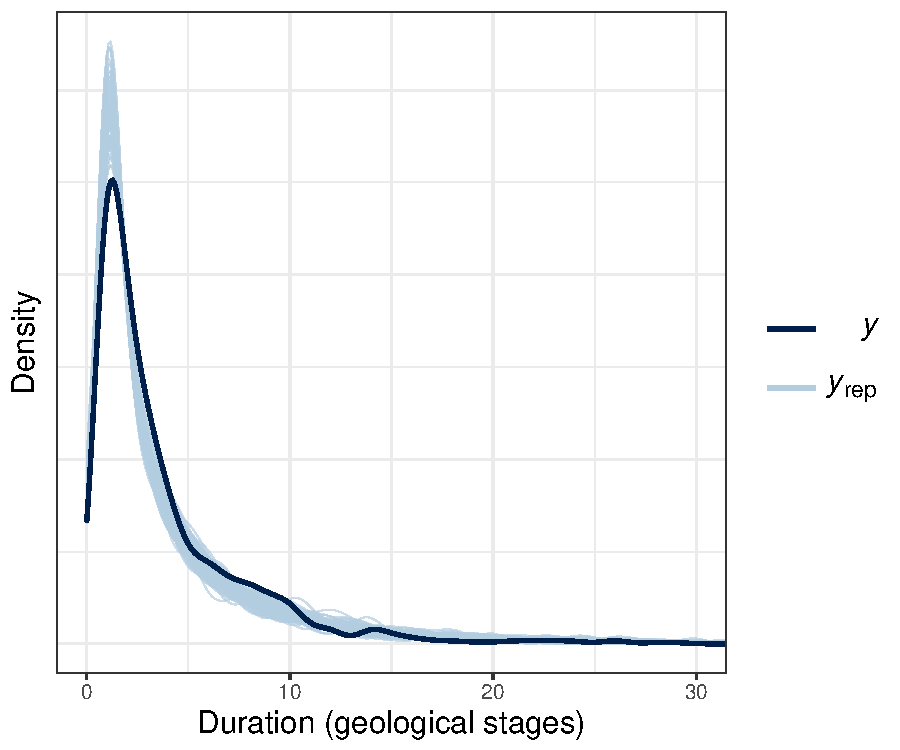
\includegraphics[height = 0.5\textheight,width=\textwidth,keepaspectratio=true]{figure/ppc_dens_zoom_cweib_cens}
  \caption{ Comparison of the distribution of the observed data (black) to 100 simulated distributions (blue). This is a close-up view of the bulk of the distribution which shows the more subtle aspects of (mis)fit between the data and the model. }
  \label{fig:dens_overlay_zoom}
\end{figure}

\begin{figure}[ht]
  \centering
  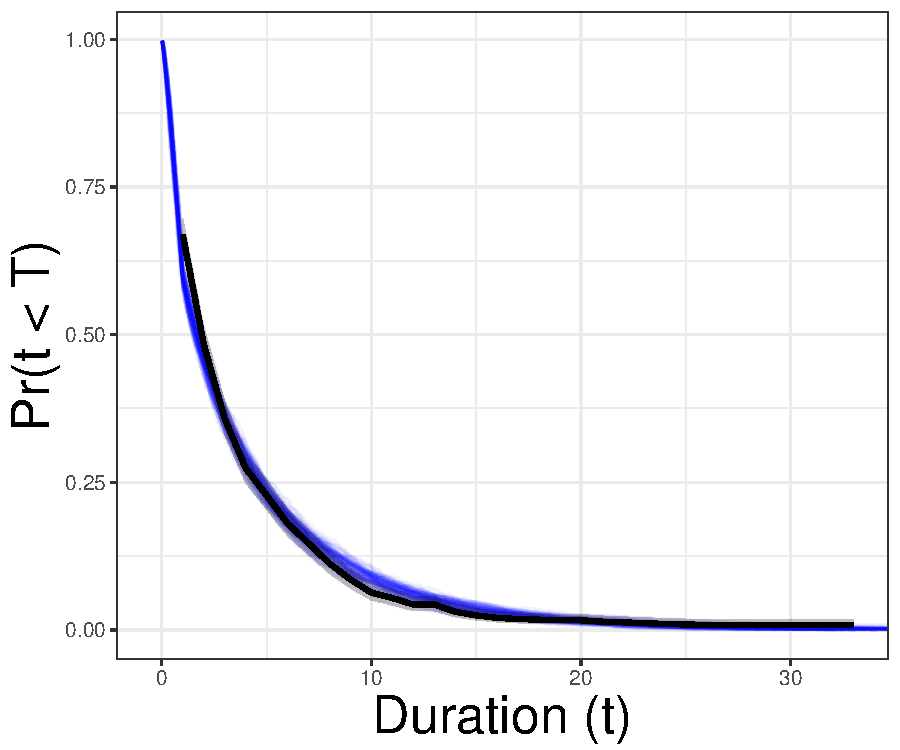
\includegraphics[height = 0.5\textheight,width=\textwidth,keepaspectratio=true]{figure/survival_curves_cweib_cens}
  \caption{Comparison of the empirical estimate of \(S(t)\) (blue) versus estimates from 100 posterior predictive data sets (black). \(S(t)\) corresponds to the probability that the age of a genus \(t\) is less than the genus' ultimate duration \(T\). }
  \label{fig:surv}
\end{figure}

\begin{figure}[ht]
  \centering
  \begin{subfigure}{0.4\textwidth}
    \caption{}
    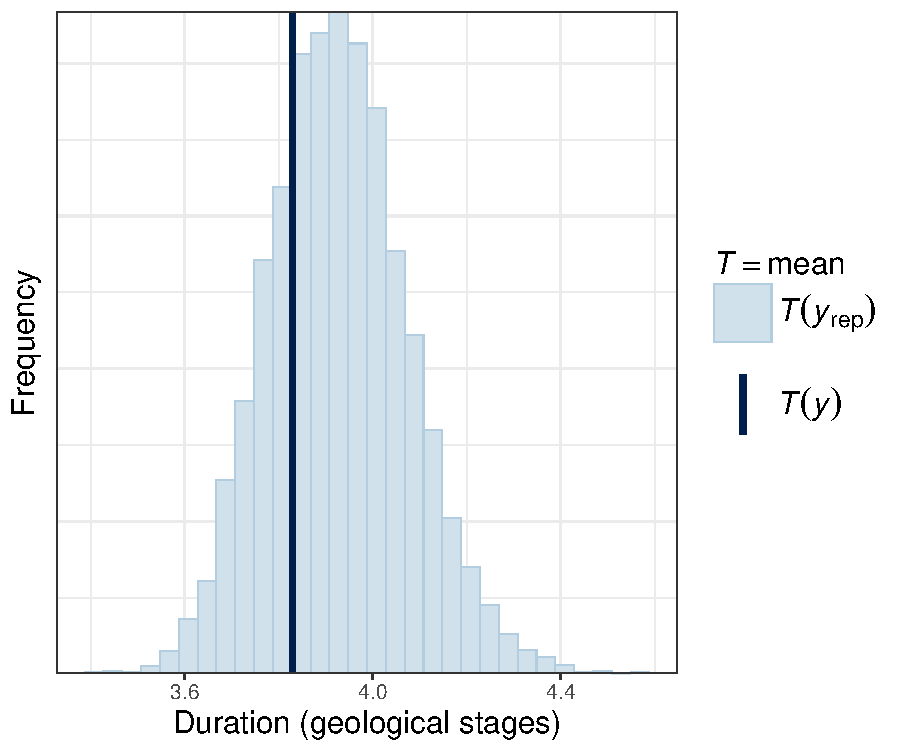
\includegraphics[height = 0.5\textheight,width=0.9\textwidth,keepaspectratio=true]{figure/ppc_mean_cweib_cens}
    \label{fig:ppc_mean}
  \end{subfigure}
  \begin{subfigure}{0.4\textwidth}
    \caption{}
    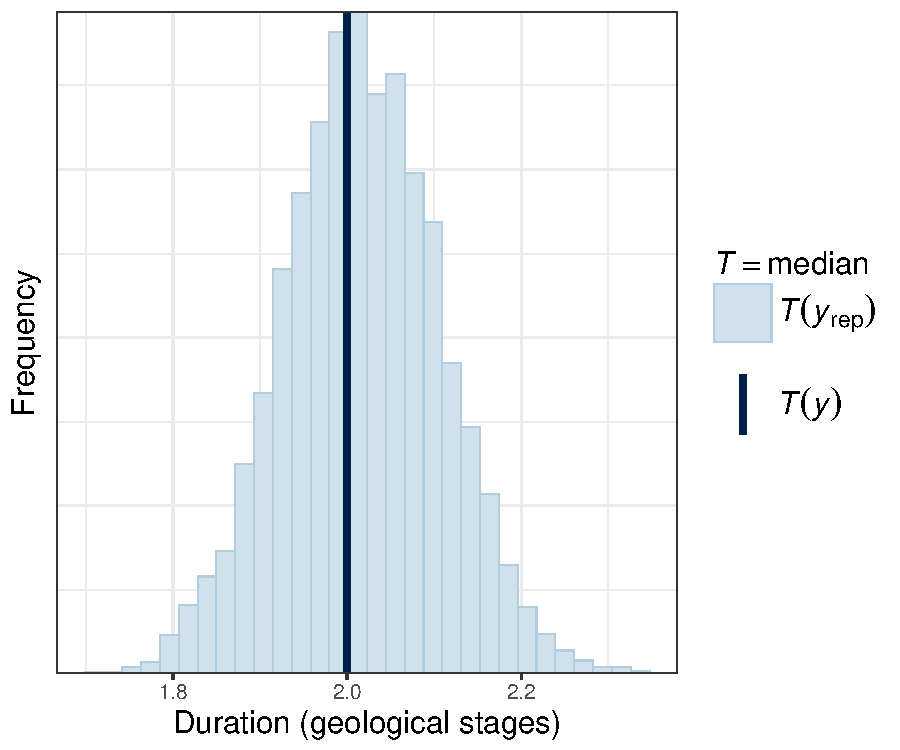
\includegraphics[height = 0.5\textheight,width=0.9\textwidth,keepaspectratio=true]{figure/ppc_median_cweib_cens}
    \label{fig:ppc_median}
  \end{subfigure}
  \caption{ Comparison of the (A) observed mean genus duration (black vertical line) to a distribution of means estimated from 100 simulated datasets (blue), and (B) comparison of the observed median genus duration (black vertical line) to a distribution of medians estimated from 100 simulated datasets (blue). Model fit is evaluated by the similarity between the observed and the estimated, where good fit is demonstrated by the vertical line being ``within'' the simulated distribution. }
  \label{fig:points}
\end{figure}


\begin{figure}[ht]
  \centering
  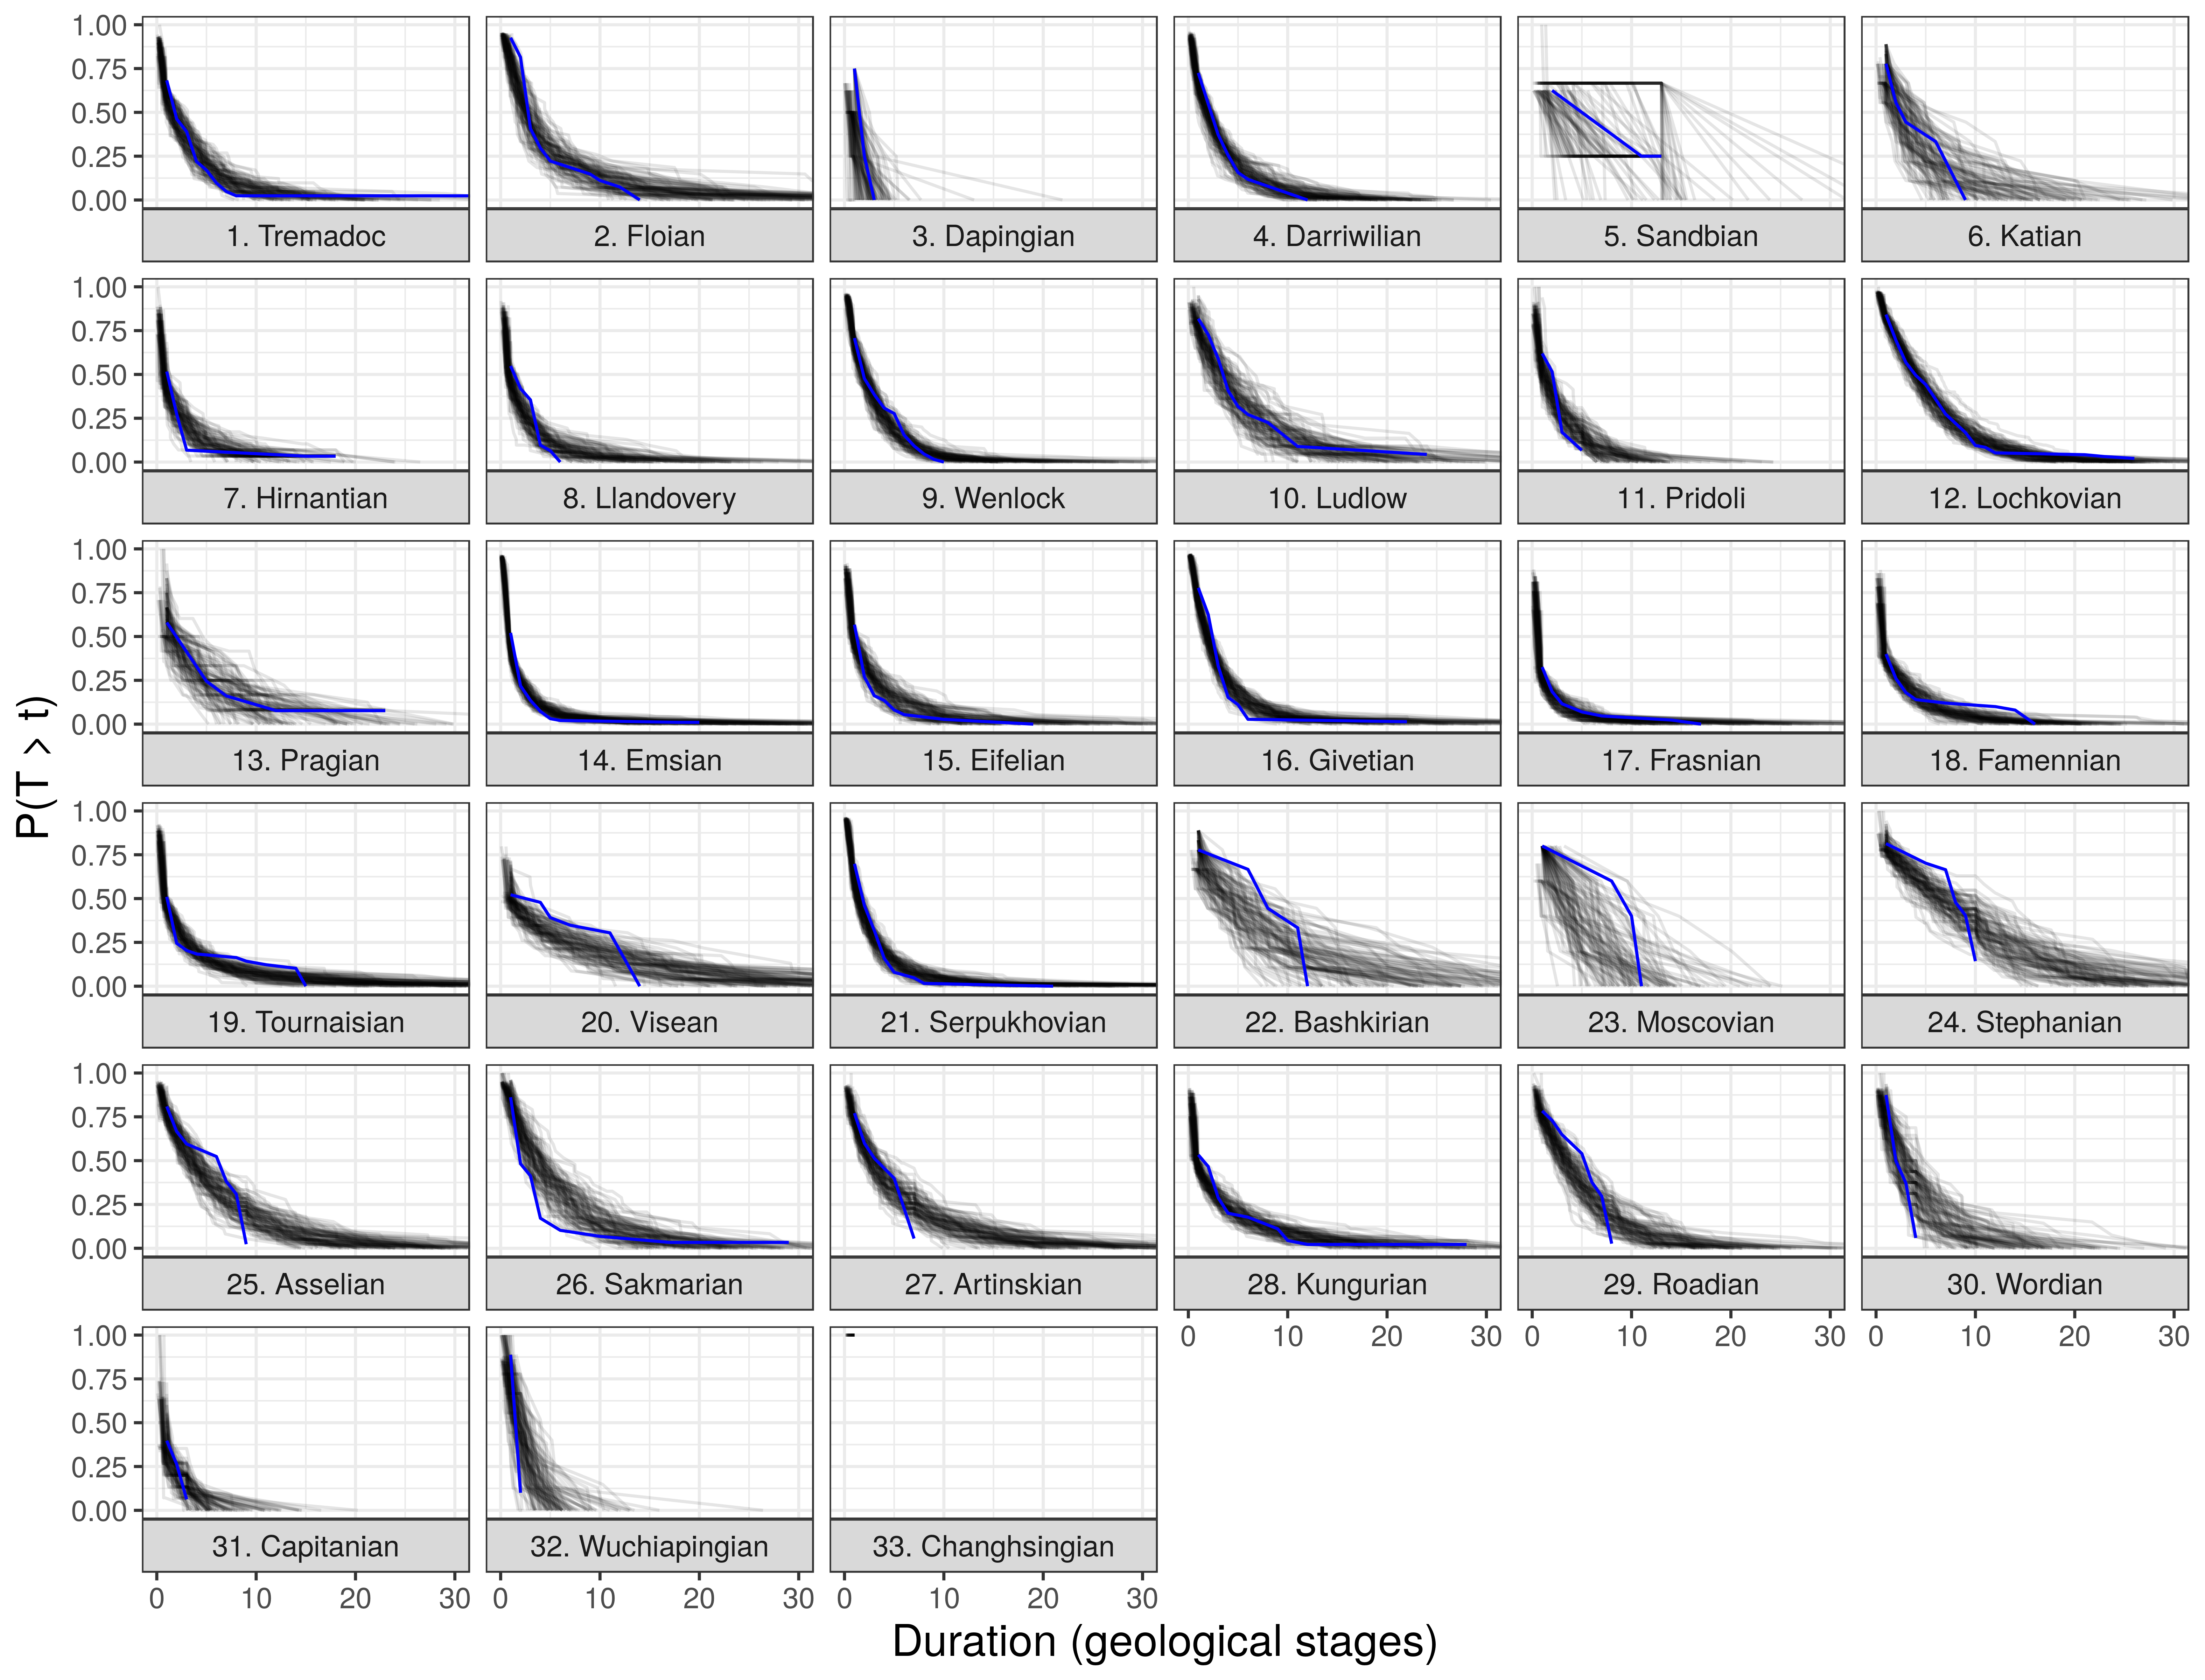
\includegraphics[height = 0.5\textheight,width=\textwidth,keepaspectratio=true]{figure/ppc_surv_coh}
  \caption{Comparison of the empirical estimate of \(S(t)\) (blue) versus estimates from 100 posterior predictive data sets (black) for each of the origination cohorts. \(S(t)\) corresponds to the probability that the age of a genus \(t\) is less than the genus' ultimate duration \(T\). By comparing the fit of the model to the individual cohorts, when and where the model (mis)fits is more observable. }
  \label{fig:surv_group}
\end{figure}

\begin{figure}[ht]
  \centering
  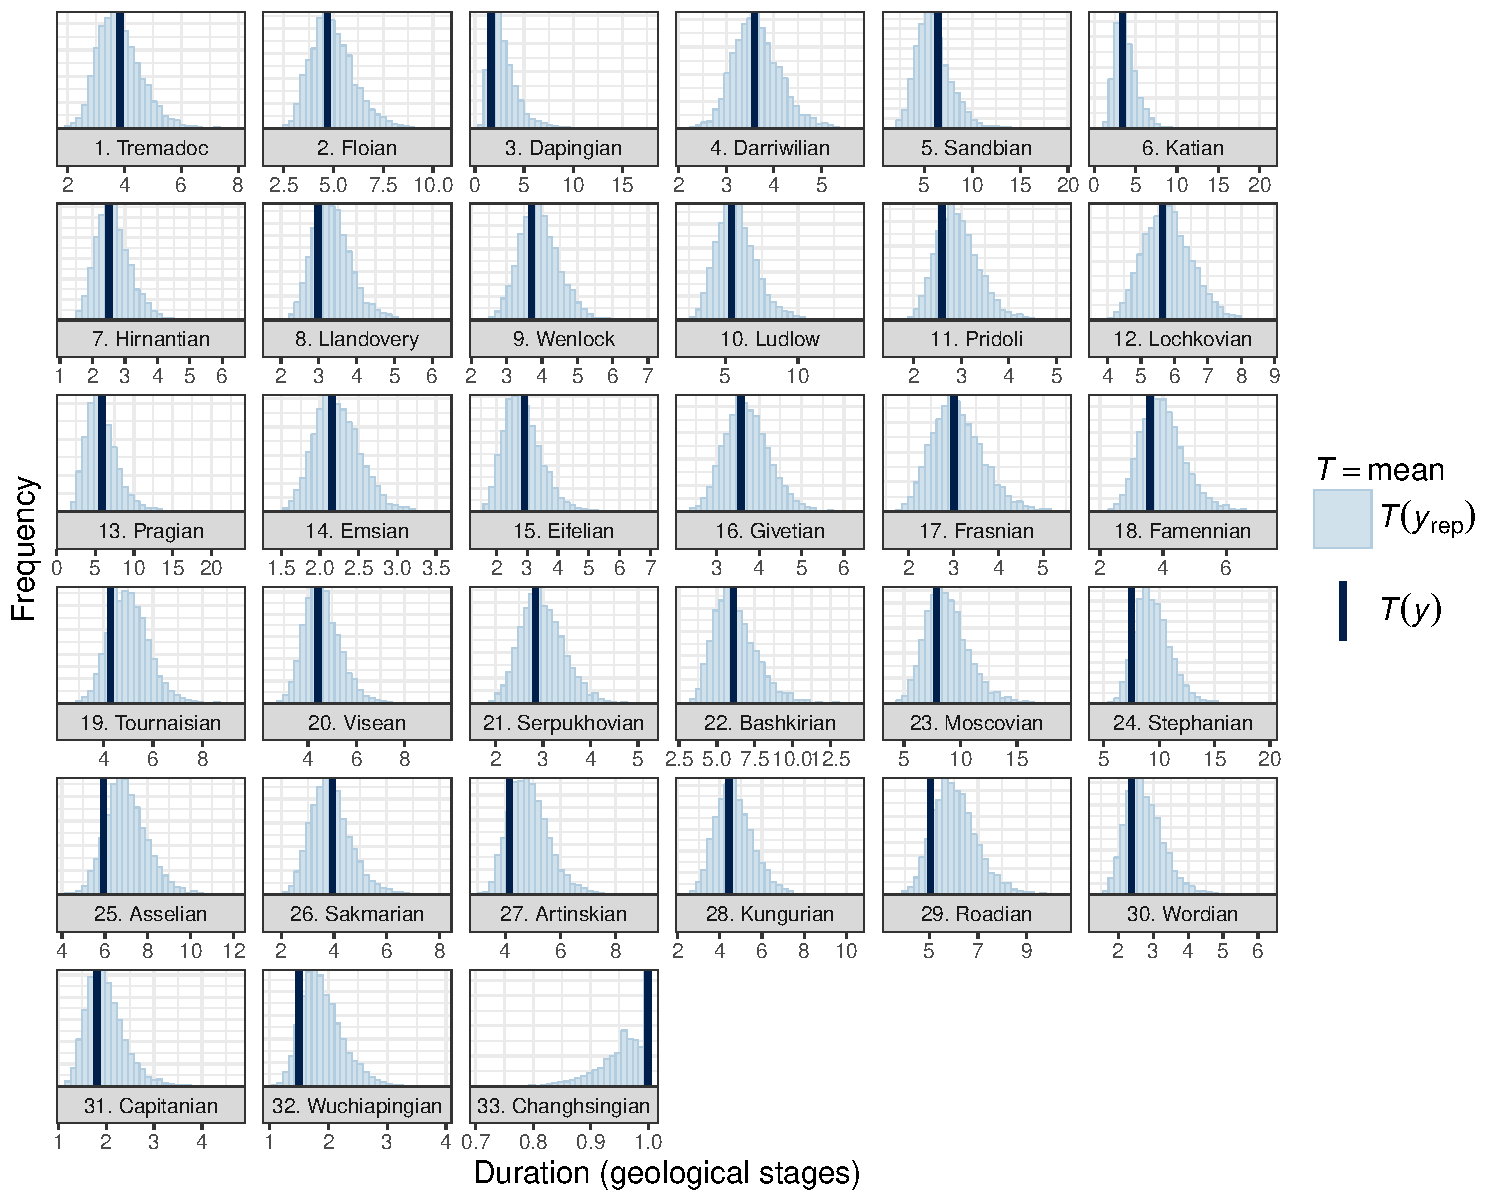
\includegraphics[height = 0.5\textheight,width=\textwidth,keepaspectratio=true]{figure/ppc_mean_group_cweib_cens}
  \caption{ Comparison of the observed mean genus duration (black vertical line) to a distribution of means estimated from 100 simulated datasets (blue) for each of the origination cohorts. Model fit is evaluated by the similarity between the observed and the estimated, where good fit is demonstrated by the vertical line being ``within'' the simulated distribution. }
  \label{fig:group_mean}
\end{figure}

\begin{figure}[ht]
  \centering
  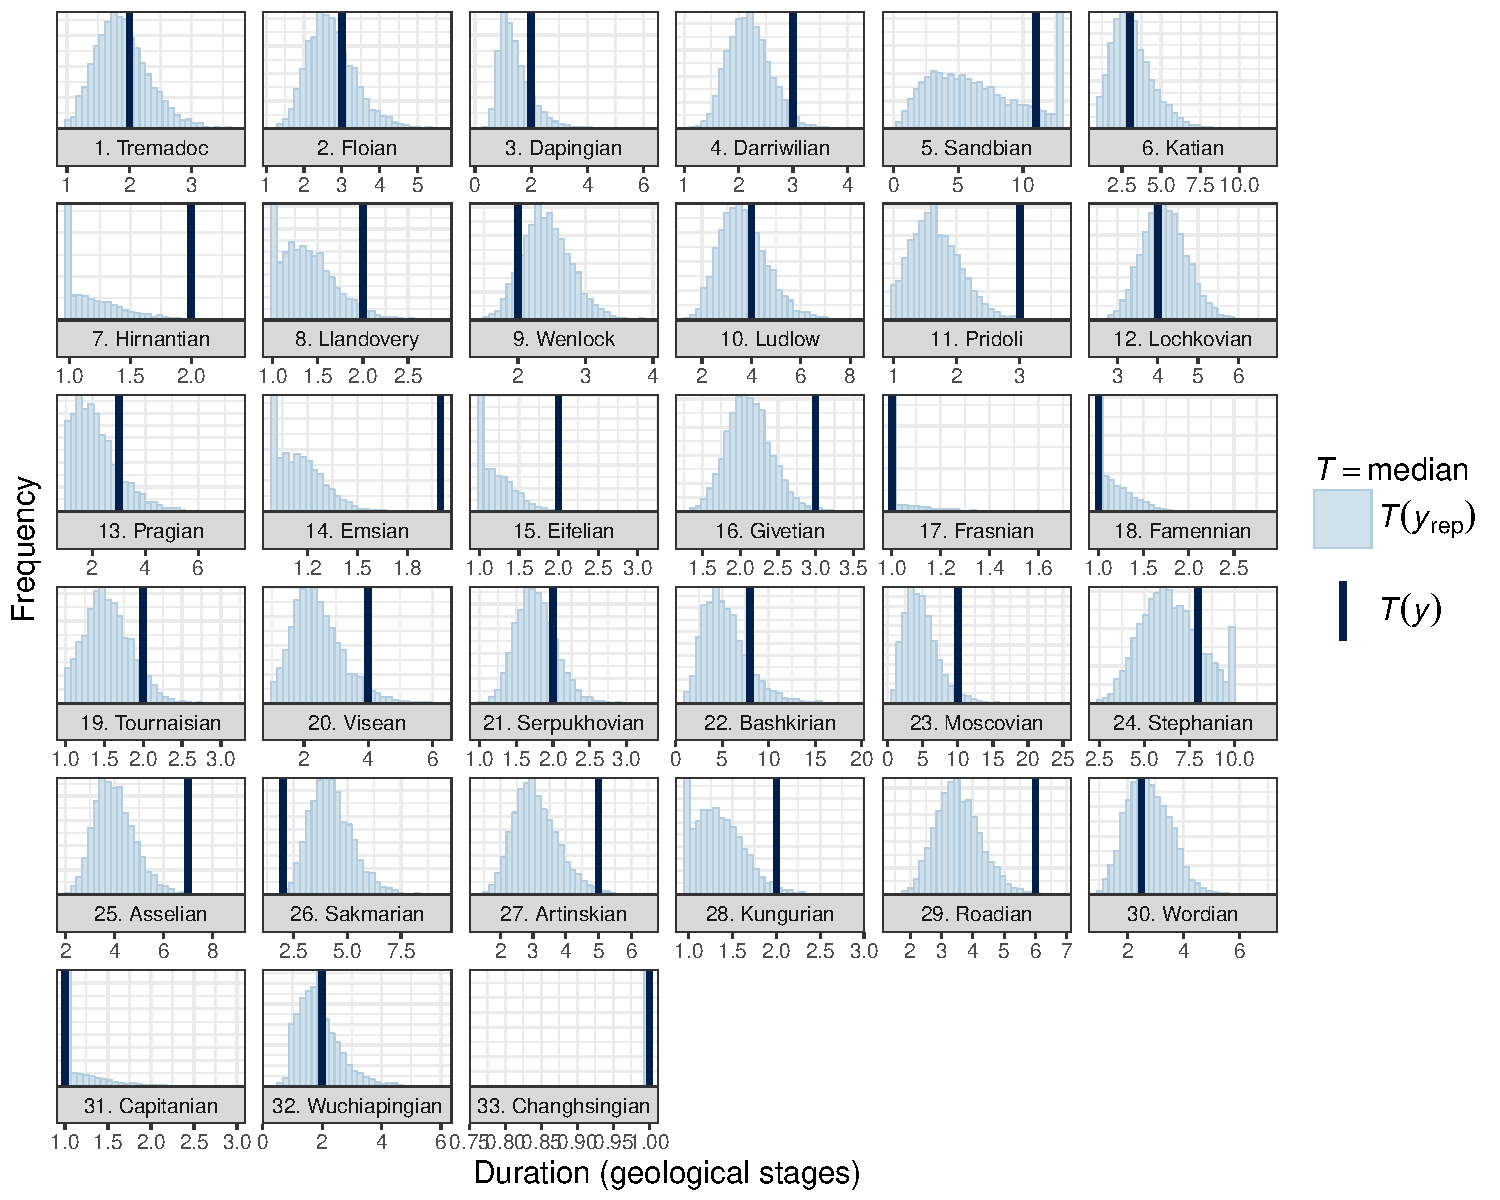
\includegraphics[height = 0.5\textheight,width=\textwidth,keepaspectratio=true]{figure/ppc_med_group_cweib_cens}
  \caption{ Comparison of the observed median genus duration (black vertical line) to a distribution of medians estimated from 100 simulated datasets (blue) for each of the origination cohorts. Model fit is evaluated by the similarity between the observed and the estimated, where good fit is demonstrated by the vertical line being ``within'' the simulated distribution. }
  \label{fig:group_median}
\end{figure}

\begin{figure}[ht]
  \centering
  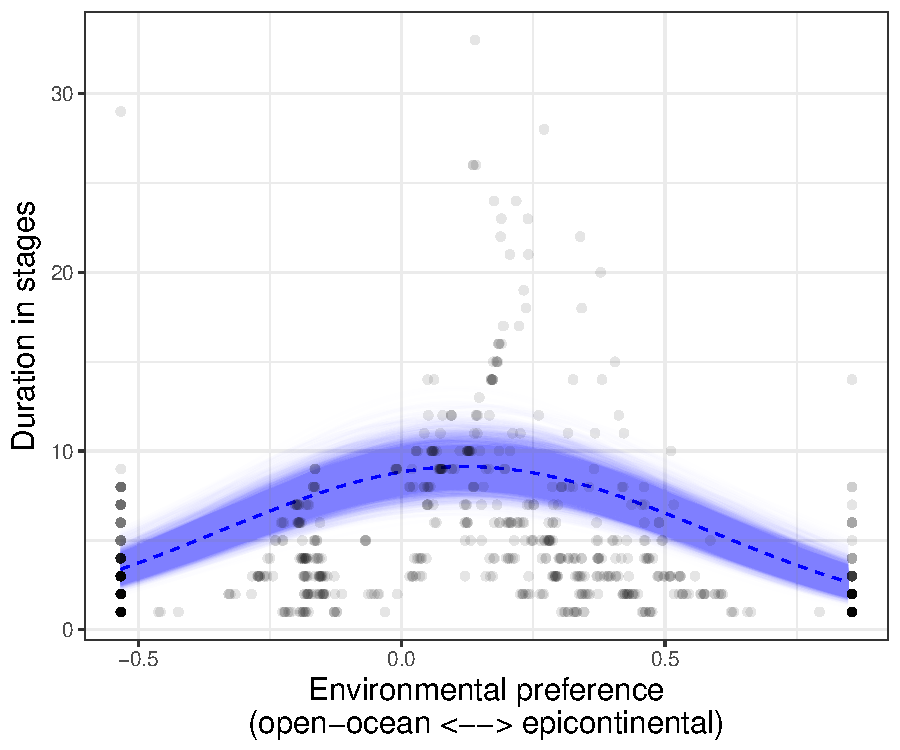
\includegraphics[height = 0.5\textheight,width=\textwidth,keepaspectratio=true]{figure/env_effect_med_cweib_cens}
  \caption{The overall expected relationship between environmental affinity \(v_{i}\) and a \(\log(\sigma)\) when r = 0 and m = 0. The 1000 semi-transparent lines corresponds to a single draw from the posterior predictive distribution, while the highlighted line corresponds to the median of the posterior predictive distribution. The overall relationship demonstrates a greater durations among environmental generalists than specialists. Additionally, because the apex of is rightward from 0, taxa favoring epicontinental environments are expected to have a slightly longer durations than those favoring open-ocean environments. The tick marks along the bottom of the plot correspond to the (rescaled) observed values of environmental preference.}
  \label{fig:env_mean}
\end{figure}

\begin{figure}[ht]
  \centering
  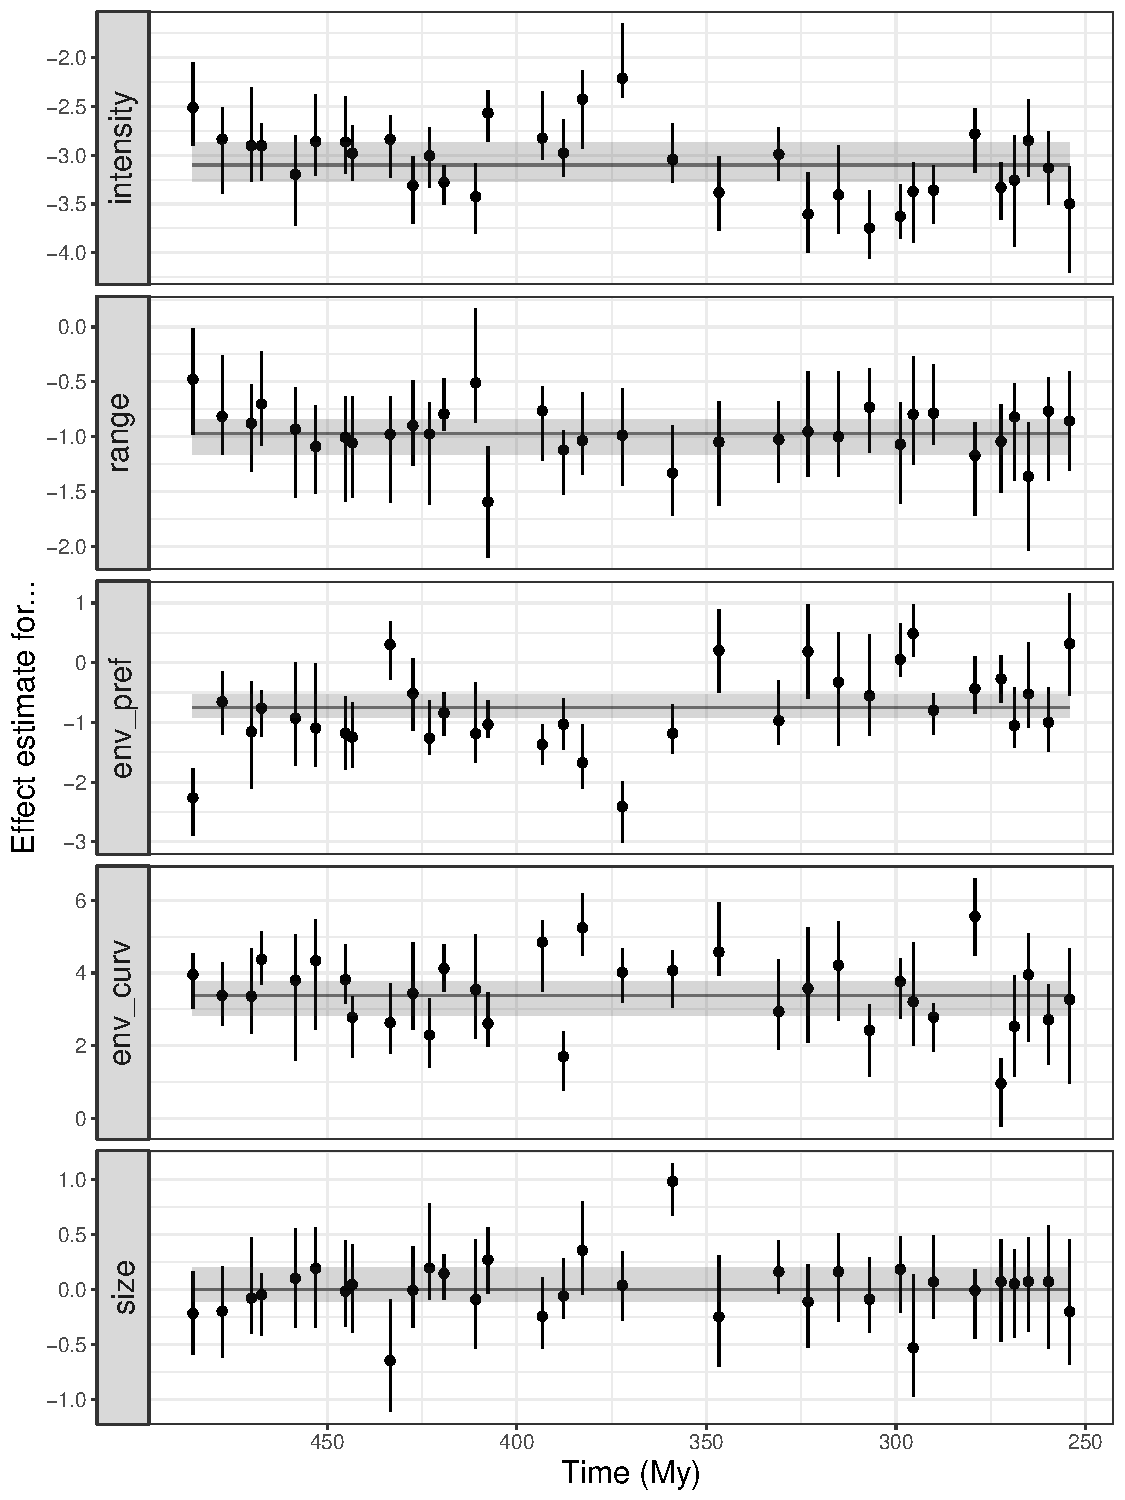
\includegraphics[width = \textwidth,height = 0.7\textheight,keepaspectratio=true]{figure/cohort_series_cweib_cens}
  \caption{Comparison of cohort-specific estimates of \(\beta^{0}\), the effect of geographic range on extinction risk \(\beta^{r}\), the effect of environmental preference \(\beta^{v}\) and \(\beta^{v^{2}}\), and body size \(\beta^{m}\). Points correspond to the median of the cohort-specific estimate, along with 80\% credible intervals. Points are plotted at the midpoint of the cohorts stage of origination in millions of years before present (My). Black, horizontal lines are the overall estimates of covariate effects along with 80\% credible intervals (shaded).}
  \label{fig:cohort_series}
\end{figure}

\begin{figure}[ht]
  \centering
  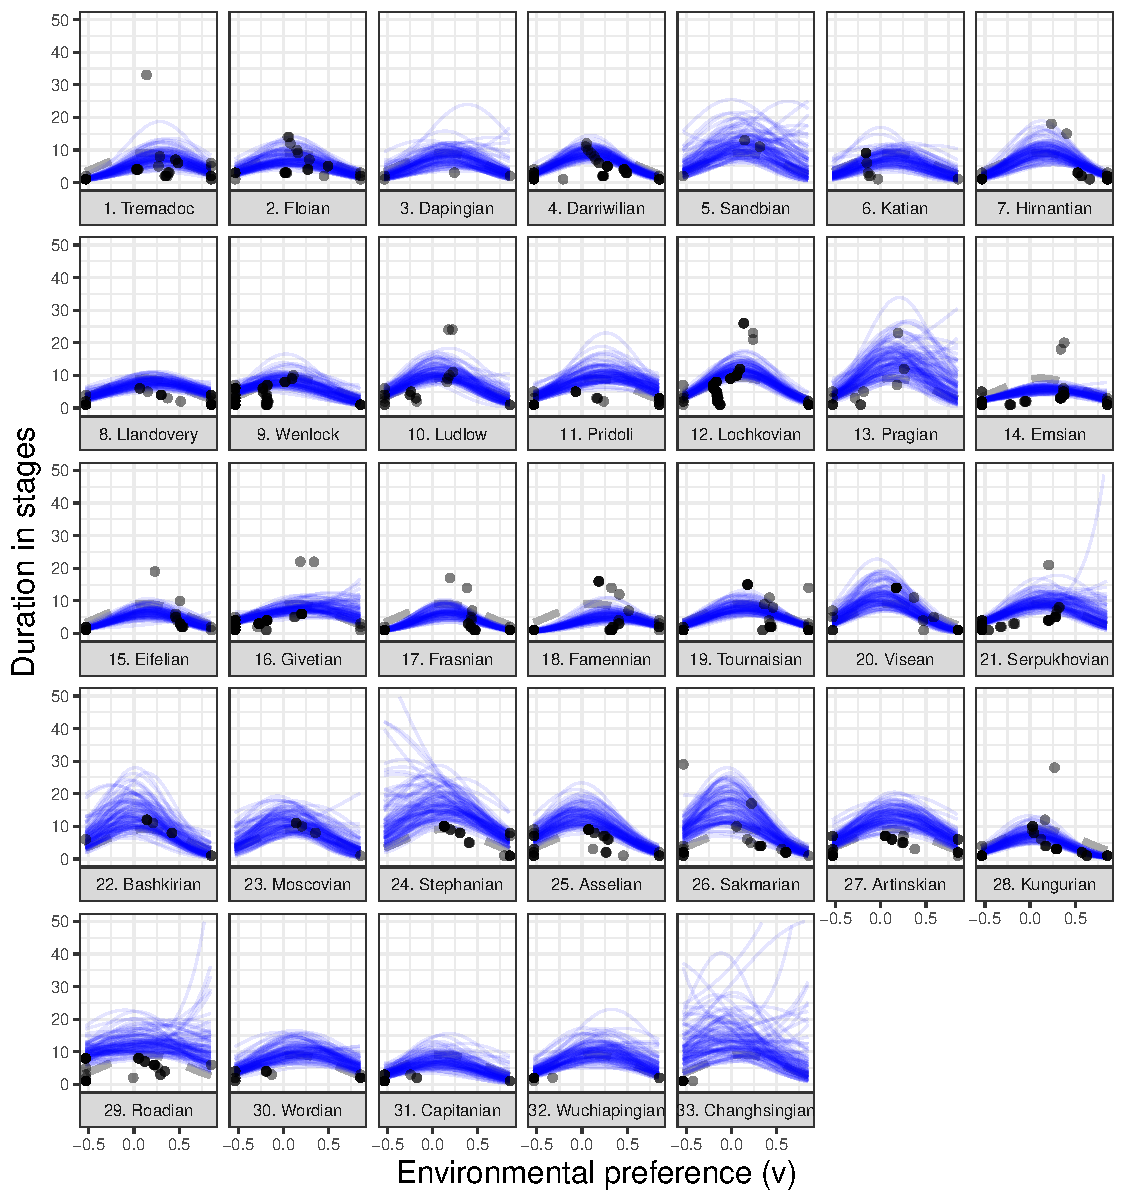
\includegraphics[width = \textwidth,height = 0.7\textheight,keepaspectratio=true]{figure/env_cohort_med_cweib_cens}
  \caption{Comparison of origination cohort-specific (posterior predictive) estimates of the effect of environmental preference on \(\log(\sigma)\) to the mean overall estimate of the effect of environmental preference. Cohort-specific estimates are from 100 posterior predictive simulations across the range of (transformed and rescaled) observed values of environmental preference. The oldest cohort is in the top-left and younger cohorts proceed left to right, with the youngest cohort being the right-most facet of the last row. Panel names correspond to the name of the stage in which that cohort originated.}
  \label{fig:env_cohort}
\end{figure}

\begin{figure}[ht]
  \centering
  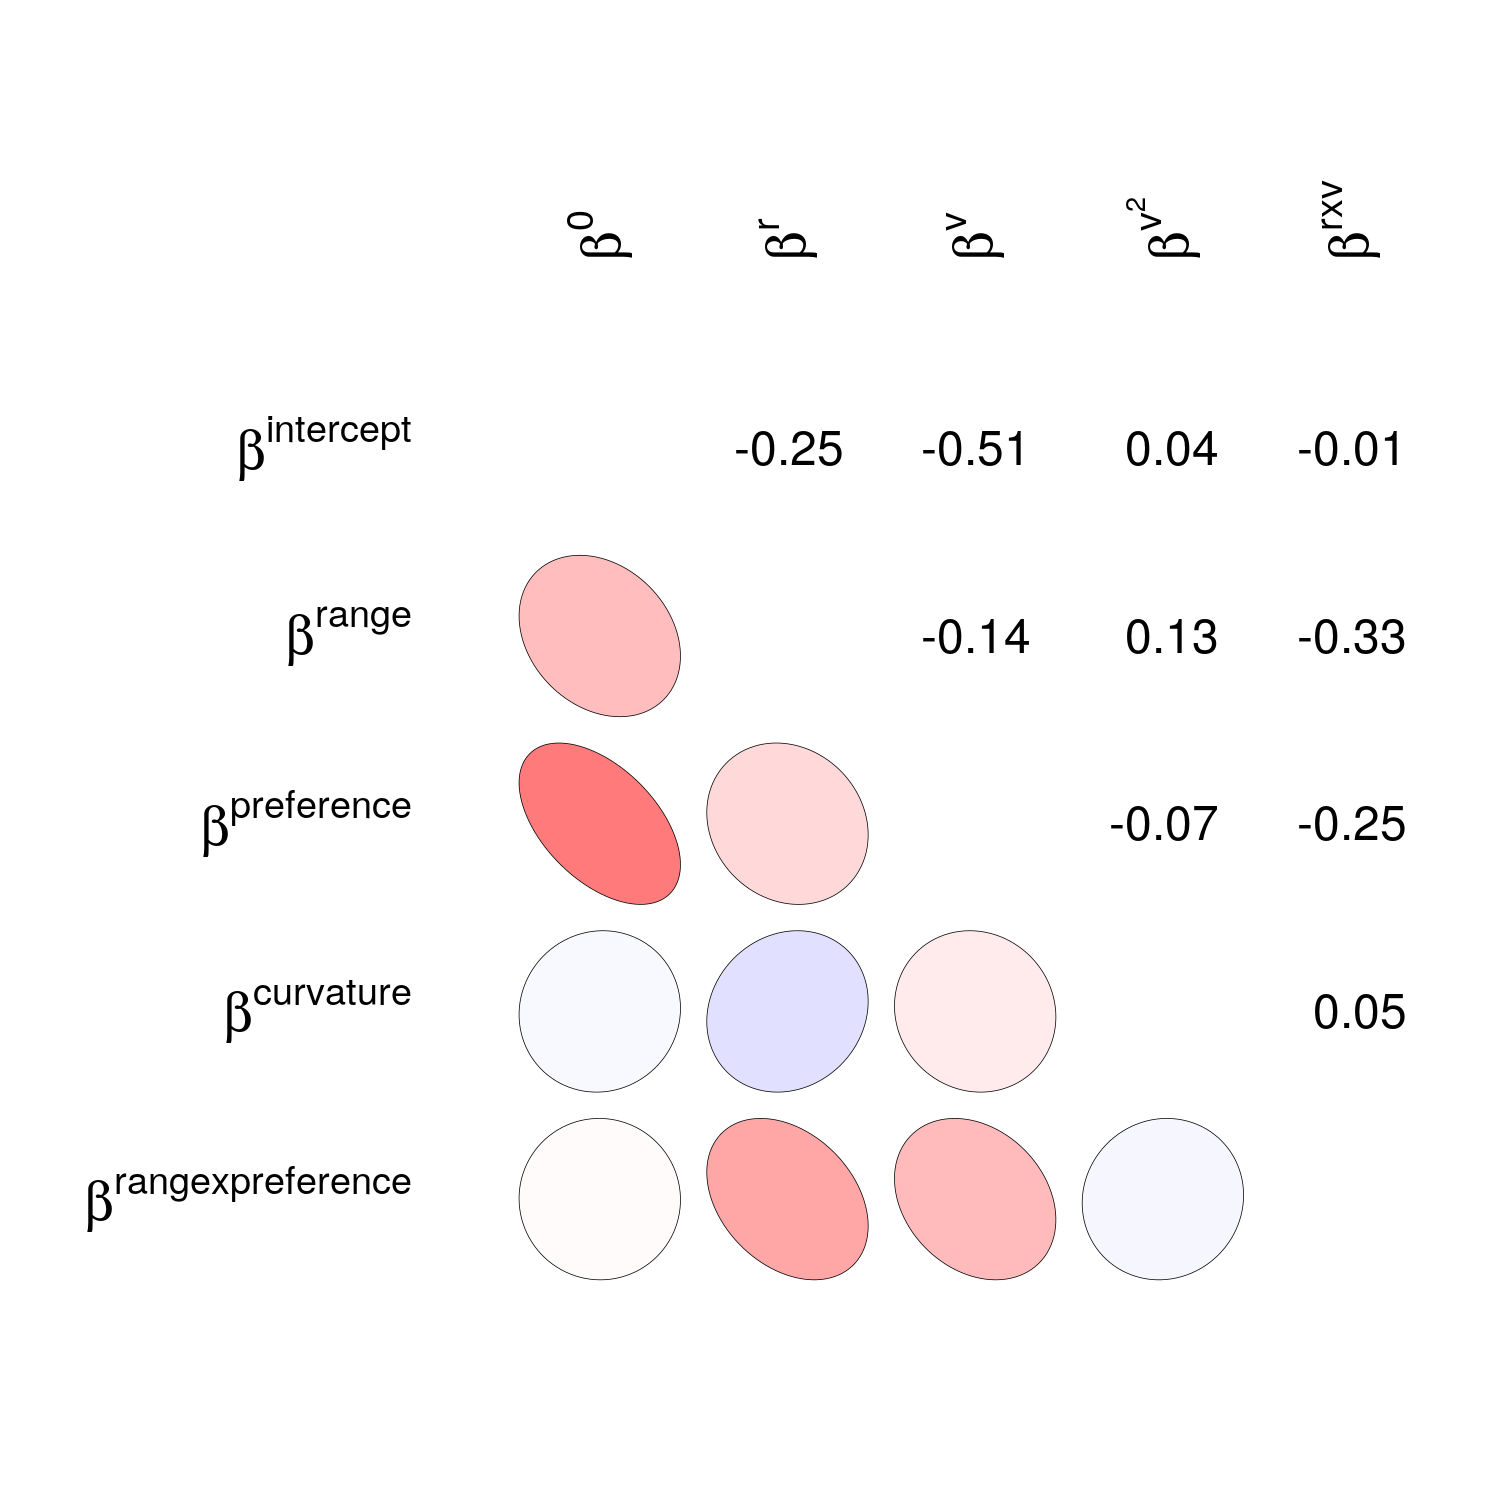
\includegraphics[height = 0.7\textheight,width=\textwidth,keepaspectratio=true]{figure/wei_cor_heatmap_cweib_cens}
  \caption{Mixed graphical and numerical representation of the correlation matrix \(\Omega\) of variation in cohort-specific covariate estimates. These correlations are between the estimates of the cohort-level effects of covariates, along with intercept/baseline extinction risk. The median estimates of the correlations are presented numerically (upper-triangle) and as idealized ellipses representing that much correlation (lower-triangle). The darkness of the ellipse corresponds to the magnitude of the correlation.}
  \label{fig:cor_posterior}
\end{figure}



\end{document}
